\chapter{The Helly property and EPG graphs}\label{cap:capiii}

\begin{flushright}
\begin{minipage}[t][0cm][b]{0.47\textwidth}
\emph{
Talento é 1\% inspiração e 99\% transpiração. }
\end{minipage}

\rule[0cm]{7cm}{0.03cm}%{largura}{espessura}

Thomas Edison
\end{flushright}

% Neste capítulo examinaremos as relações hierárquicas entre algumas classes EPG e EPG-Helly. Ademais, abordaremos representações $B_1$-EPG de alguns grafos que serão utilizados posteriormente. Primeiro, vamos observar como as classes $B_0$-EPG, $B_0$-EPG-Helly, $B_1$-EPG e $B_1$-EPG-Helly se relacionam, em seguida consideramos as representações $B_1$-EPG de $C_4$'s e do grafo octaedro. Por último, apresentaremos a prova de $NP$-completude do problema de reconhecimento de grafos $B_1$-EPG-Helly.

In this chapter we will examine the hierarchical relationships between some EPG and Helly-EPG classes. In addition, we will approach $ B_1$-EPG representations of some graphs that will be used later. First, let is focus our attention to understand how the classes $B_0$-EPG, $B_1$-EPG,  Helly-$B_1$ EPG and  $L$-shaped paths are related, then we consider the $ B_1$-EPG representations of graphs $C_4 $ and the Octahedral graph. Next, we will present the proof of $NP$-completeness to Helly-$B_1$-EPG graph recognition problem. Finally, at the end of this chapter the reader can find a section with a complete version of the paper published in the journal DMTCS that contains the set of proofs that have been omitted from the text.


\section{Introduction}
An EPG graph $G$ is a graph that admits a representation in which its vertices are represented by paths of a grid $Q$, such that two vertices of $G$ are adjacent if and only if the corresponding paths have at least one common edge.

The study of EPG graphs has motivation related to the problem of VLSI design that combines the notion of edge intersection graphs of paths in a  tree with a  VLSI  grid layout model, see~\cite{golumbic2009}. The number of bends in an integrated circuit may increase the layout area, and consequently, increase the cost of chip manufacturing.
This is one of the main applications that instigate research on the EPG representations of some graph families when there are constraints on the number of bends in the paths used in the representation.
Other applications and details on circuit layout problems can be found in~\cite{bandy1990, molitor1991}.

A graph is a $ B_k$-EPG graph if it admits a representation in which each path has at most $k$ bends. As an example, Figure~\ref{fig:trianguloepgRepresentacao}(a) shows a $C_3$, Figure~\ref{fig:trianguloepgRepresentacao}(b) shows an EPG representation where the paths have no bends and Figure~\ref{fig:trianguloepgRepresentacao}(c) shows a representation with at most one bend per path.   
Consequently, $C_3$ is a $B_0$-EPG graph. More generally, $B_0$-EPG graphs coincide with interval graphs.


\begin{figure}[h]
  \centering
  \begin{tabular}{ p{3cm} p{0.7cm} p{4cm} p{0.7cm} p{4cm} }
    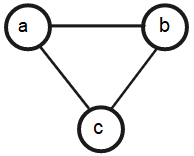
\includegraphics[width=2.3cm]{./img/trianguloabc} && 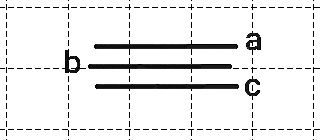
\includegraphics[width=3.9cm]{./img/b0epgTransparenciaGrade2} & &
    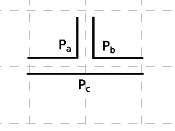
\includegraphics[width=3.5cm]{./img/b1EpgTransparenteGrade2}
    \\
    \footnotesize
    (a) The  graph $C_3$. && \footnotesize(b) $B_0$-EPG representation of $C_3$ (edge-clique).&& \footnotesize(c) $B_1$-EPG representation of $C_3$ (claw-clique).\\
  \end{tabular}

 \caption{The  graph $ C_3 $  and  representations without bends and with 1 bend.} \label{fig:trianguloepgRepresentacao}
\end{figure}


The \emph{bend number} of a graph $G$ is the smallest $k$ for which $G$ is a $B_k$-EPG graph. Analogously, the bend number of a class of graphs is the smallest $k$ for which all graphs in the class have a $B_k$-EPG representation. Interval graphs have bend number $0$, trees have bend number $1$, see~\cite{golumbic2009}, and outerplanar graphs have bend number $2$, see~\cite{daniel2014b}. The bend number for the class of planar graphs is still open, but according to \cite{daniel2014b}, it is either $3$ or $4$.

The class of EPG graphs has been studied in several papers, such as \cite{alcon2016, Asinowski2009, cohen2014, golumbic2009, heldt2014,  martin2017,golumbic2019edge}, among others. The investigations regarding EPG graphs frequently approach characterizations concerning the number of bends of the graph representations. Regarding the complexity of recognizing $B_k$-EPG graphs, only the complexity of recognizing a few of these sub-classes of EPG graphs have been determined: $B_0$-EPG graphs can be recognized in polynomial time, since it corresponds to the class of interval graphs, see ~\cite{booth1976}; in contrast, recognizing $B_1$-EPG and $B_2$-EPG graphs are NP-complete problems, see~\cite{heldt2014} and \cite{martin2017}, respectively. 
Also, note that the paths in a $B_1$-EPG representation have one of the following shapes: $\llcorner$, $\lrcorner$, $\ulcorner$ and $\urcorner$. \cite{cameron2016edge} showed that for each $S\subset \{\llcorner, \lrcorner, \ulcorner, \urcorner\}$, it is NP-complete to determine if a given graph $G$ has a $B_1$-EPG representation using only paths with shape in $S$.

A  collection $C$ of sets satisfies the Helly property when every sub-collection of $C$ that is pairwise intersecting has at least one common element. 
The study of the Helly property is useful in diverse areas of science. We can enumerate applications in semantics, code theory, computational biology, database, image processing, graph theory, optimization, and linear programming, see \cite{dourado2009}.

The Helly property can also be applied to the $B_k$-EPG representation problem, where each path is considered a set of edges. A graph $G$ has a  Helly-$B_k$-EPG representation if there is a $B_k$-EPG representation of $G$ where each path has at most $k$ bends, and this representation satisfies the Helly property. Figure~\ref{fig:envelopeRepresentacoes}(a) presents two $B_1$-EPG representations of a graph with five vertices.  Figure~\ref{fig:envelopeRepresentacoes}(b)   illustrates 3 pairwise intersecting paths ($P_{v_1}, P_{v_2}, P_{v_5}$), containing a common edge, so it is a Helly-$B_1$-EPG representation. In Figure~\ref{fig:envelopeRepresentacoes}(c), although the three paths are pairwise intersecting, there is no common edge in all three paths, and therefore they do not satisfy the Helly property.

The Helly property related to EPG representations of graphs has been studied in~\cite{golumbic2009} and~\cite{golumbic2013}. 

Let $\cal {F}$ be a family of subsets of some universal set $U$, and $h\geq 2$ be an integer.  Say that $\cal{F}$ is $h$-{\it intersecting} when every group of $h$ sets of $\cal {F}$ intersect. The {\it core} of $\cal {F}$, denoted by $core(\cal F)$, is the intersection of all sets of $\cal {F}$. The family $\cal{F}$ is $h$-{\it Helly} when every $h$-intersecting subfamily $\cal{F'}$ of $\cal{F}$ satisfies $core(\cal{F'}) \neq \emptyset$, see e.g. \cite{D76}. On the other hand, if for every subfamily $\cal{F'}$ of $\cal{F}$, there are $h$ subsets whose core equals the core of  $\cal {F'}$, then $\cal {F}$ is said to be {\it strong} $h$-{\it Helly}.
Note that the Helly property that we will consider in this paper is precisely the property of being 2-Helly. 

The  {\it Helly number} of the family $\cal{F}$ is the least integer $h$, such that $\cal{F}$ is $h$-Helly. Similarly, the {\it strong Helly number} of $\cal{F}$ is the least $h$, for which  $\cal{F}$ is strong $h$-Helly. It also follows that the strong Helly number of $\cal{F}$ is at least equal to its Helly number. In~\cite{golumbic2009} and~\cite{golumbic2013}, they have determined the strong Helly number of $B_1$-EPG graphs. 


\begin{figure}[h]
  \centering
  \begin{tabular}{ p{3.2cm} p{4.5cm} p{4.5cm} }
    \centering 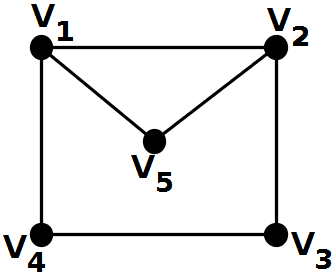
\includegraphics[width=3cm]{./img/envelope} & 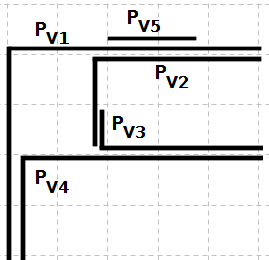
\includegraphics[width=4cm]{./img/envelopeHellyGradeTransparente} & 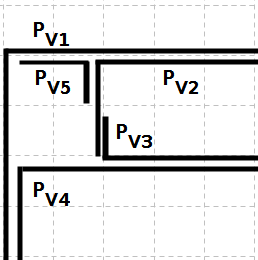
\includegraphics[width=4cm]{./img/envelopeNaoHellyGrade}
    \\
    \footnotesize \centering (a) A  graph with 5 vertices. & \footnotesize(b) A $B_1$-EPG representation that satisfies the Helly property. & \footnotesize (c) A $B_1$-EPG representation that does  not satisfy the Helly property.  \\

  \end{tabular}
\caption{A  graph with 5 vertices in (a) and some single bend representations: Helly in (b) and not Helly in (c).} \label{fig:envelopeRepresentacoes}
\end{figure}

%%%%%%%%%%%%%%%%%%%%%%%%%%%%%%%%%%%%%%%%%%%%%%%%%%%%%%%%%%%%%


Next, we describe some terminology and notation.

The term \emph{grid} is used to denote the Euclidean space of integer orthogonal coordinates. Each pair of integer coordinates corresponds to a \emph{point} (or vertex) of the grid. The \emph{size} of a grid is its number of points. The term \emph{edge of the grid} will be used to denote a pair of vertices that are at a distance one in the grid. Two edges $e_1$ and $e_2$ are \emph{consecutive edges} when they share exactly one point of the grid.
 A (simple) path in the grid is as a sequence of distinct edges $e_1, e_2, \leq, e_m$,  where consecutive edges are adjacent, i.e., contain a common vertex, whereas non-consecutive edges are not adjacent.  In this context, two paths only intersect if they have at least a common edge. The first and last edges of a path are called \emph{extremity edges}.
  
The \emph{direction of an edge} is vertical when the first coordinates of its vertices are equal, and is horizontal when the second coordinates are equal. A \emph {bend} in a path is a pair of consecutive edges $ e_1, e_2 $ of that path, such that the directions of $ e_1$ and $ e_2$ are different. When two edges $ e_1$ and $e_2 $ form a bend, they are called \emph { bend edges}. A \emph {segment} is a set of consecutive edges with no bends. %is a path with no bends.
Two paths are said to be \emph{edge-intersecting}, or simply  \emph{intersecting} if they share at least one edge. Throughout the paper, any time we say that two paths intersect, we mean that they edge-intersect. If every path in a representation of a graph $G$ has at most $k$ bends, we say that this graph $G$ has a \emph{$B_k$-EPG} representation. When $k = 1$ we say that this is a \emph{single bend} representation.

\medskip

In this chapter, we study the Helly-$B_k$-EPG graphs. First, we show that every graph admits an EPG representation that is Helly, and present a characterization of Helly-$B_1$-EPG representations. Besides, we relate Helly-$B_1$-EPG graphs with L-shaped graphs, a natural family of subclasses of $B_1$-EPG. Finally, we prove that recognizing Helly-$B_k$-EPG graphs is in NP, for every fixed $k$. Besides, we show that recognizing Helly-$B_1$-EPG graphs is NP-complete, and it remains NP-complete even when restricted to 2-apex and 3-degenerate graphs.

The rest of the chapter is organized as follows. In Section~\ref{sec:prelim}, we present some preliminary results, we show that every graph is a Helly-EPG graph, present a characterization of Helly-$B_1$-EPG representations, and relate Helly-$B_1$ EPG with L-shaped graphs. In Section~\ref{sec:NPpert}, we discuss the NP-membership of {\sc Helly-$B_k$ EPG Recognition}. In Section~\ref{sec:sectionDispositivoClausula}, we present the NP-completeness of recognizing Helly-$B_1$-EPG graphs. Finally, in the last section the reader can find the complete paper accepted to  journal Discrete Mathematics \& Theoretical Computer Science (DMTCS) that contains the set of proofs that have been omitted from the text.


\section{Preliminaries} \label{sec:prelim}

Before leaving for more laborious results to obtain, let us first notice a simple result. We can observe that when we do not restrict the number of bends of each path, we can show that any graph can be represented as an EPG graph.

This study starts with the following lemma.

\begin{lemma}[\citet{golumbic2009}] \label{lem:todoGrafoEpg}
 Every graph is an EPG graph.
 \end{lemma}
 
 Moreover, the same applies to EPG-Helly graphs. 
 
In an equivalent way, it is also possible to show that every graph has an EPG representation that satisfies the Helly property. An algorithm that performs this construction is presented in the Lemma~\ref{lem:todoGrafoEpgHelly}.

 \begin{lemma}\label{lem:todoGrafoEpgHelly}
 Every graph is a Helly-EPG graph.
 \end{lemma}

\begin{proof}
Let $G$ be a graph with $n$ vertices $v_1, v_2, \dots, v_n$ and $\mu$ maximal cliques $C_1, C_2, \dots , C_{\mu }$. We construct a Helly-EPG representation of $G$ using a $\mu +1\times \mu +1$ grid $Q$. 
%The rows and columns correspond to each maximal cliques and are numbered $1, 2, \dots , \mu$. 
Each maximal clique $C_i$ of $G$ is mapped to an edge of $Q$ as follow: 
\begin{itemize}
    \item if $i$ is even then the maximal clique $C_i$ is mapped to the edge in column $i$ between rows $i$ and $i+1$;
    \item if $i$ is odd then the maximal clique $C_i$ is mapped to the edge in row $i$ between columns $i$ and $i+1$.
\end{itemize}

The following describes a descendant-stair-shaped construction for the paths.
  
Let $v_l \in V(G)$ and $C_i$ be the first maximal clique containing $v_l$ according to the increasing order of their indices. If $i$ is even (resp. odd) the path $P_l$ starts in column $i$ (resp. in row $i$), in the point $(i,i)$. Then $P_l$ extends to at least the point $(i+1, i)$ (resp. $(i, i+1)$) proceeding to the until the row (resp. column) corresponding to next maximal clique of the sequence containing $v_l$, we say $C_{j}$.
At this point, we bend $P_l$, which goes to the point $(j,j)$ and repeat the process previously described. 
%
Figure~\ref{fig:gradeDemonstracao} shows the Helly-EPG representation of the octahedral graph $O_3$, according to the construction previously described.

By construction, each path travels only rows and columns corresponding with maximal cliques containing its respective vertex. And, every path crosses the edges of the grid to which your maximal cliques were mapped. Thus, the previously described construction results in an EPG representation of $G$, which is Helly since every set ${\mathcal P}$ of paths representing a maximal clique has at least one edge in its core.
\end{proof}
 
 \begin{figure}[htb]	
\center%6.3
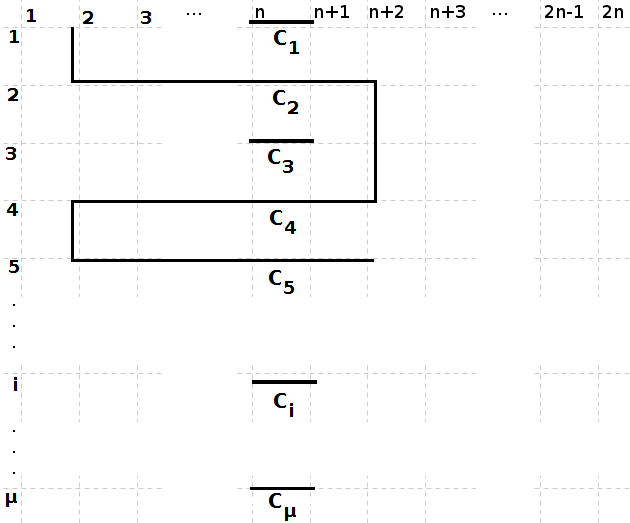
\includegraphics[width=8cm]{./img/grade3.png}
%clausulaGadgetGFCompletaSBPO
\caption{Representação do caminho $P_2$ correspondendo ao vértice $v_2$ contido nas cliques maximais $C_2, C_4$ e $C_5$}
\label{fig:gradeDemonstracao}
\end{figure}


 The provided construction in Lemma~\ref{lem:todoGrafoEpgHelly} can be modified to represent an monotonic row-ascendant EPG representation how in~\cite{golumbic2009} and~\cite{golumbic2013}. To do this, it is enough to change the orientation of the y-axis such that it grows from bottom to up.

%   The Helly property related to EPG representations of graphs has been studied in~\citet{golumbic2009,golumbic2013}.

\begin{definition}
The \emph{Helly-bend number} of a graph $G$, denoted by $b_H(G)$, is the smallest $k$ for which $G$ is a Helly-$B_k$-EPG graph. Also, the bend number of a graph class ${\mathcal C}$ is the smallest $k$ for which all graphs in ${\mathcal C}$ have a $B_k$-EPG representation.
\end{definition}
 
\begin{corollary}\label{cor:maxCliques}
For every graph $G$ containing $\mu$ maximal cliques, it holds that $b_H(G)\leq \mu -1$. 
\end{corollary}


The proof of Corollary~\ref{cor:maxCliques}  is immediate by the Lemma~\ref{lem:todoGrafoEpgHelly}.

Next, we examine the $B_1$-EPG representations of a few graphs that we employ in our constructions.

\medskip

Given an EPG representation of a graph $G$, for any grid edge $e$, the set of paths containing $e$ is a clique in $G$; such a clique is called an edge-clique. A claw in a grid consists of three grid edges meeting at a grid point. The set of paths that contain two of the three edges of a claw is a clique; such a clique is called a claw-clique, see~\cite{golumbic2009}. Fig.~\ref{fig:trianguloepgRepresentacao} illustrates an edge-clique and a claw-clique.

\begin{lemma}[\citet{golumbic2009}]\label{edge-claw-clique} 
Consider a $B_1$-EPG representation of a graph $G$. Every clique in $G$ corresponds to either an edge-clique or a claw-clique.
\end{lemma}

Next, we present a characterization of Helly-$B_1$-EPG representations.

\begin{lemma}\label{caracterization}
A $B_1$-EPG representation of a graph $G$ is Helly if and only if each clique of $G$ is represented by an edge-clique, i.e., it does not contain any claw-clique.
\end{lemma}

The Lemma~\ref{caracterization} is useful to prove that we can check if a given $B_1$-EPG representation is Helly. Just check each clique. 

Now, we consider EPG representations of $C_4$.

\begin{definition} \label{defi:tortasFrame}
Let $ Q $ be a grid and let $ (a_1, b),$ $(a_2, b),$ $(a_3, b),$ $(a_4, b)$ be a 4-star as depicted in Figure~\ref{fig:piesInGrid2}(a). Let $ \mathcal{P} = \{P_1, \dots , P_4\}$ be a collection of distinct paths each containing exactly two edges of the $4$-star.
\begin{itemize}
\item A \emph{true pie} is a representation where each $P_i$ of $ \mathcal{P} $ forms a bend in $b$.

\item A \emph {false pie} is a representation where two of the paths $P_i$ do not contain bends, while the remaining two do not share an edge. 
\end{itemize}
\end{definition}

Fig.~\ref{fig:piesInGrid2} illustrates true pie and false pie representations of a $C_4$.

\begin{figure}[htb]
  \centering
%segundo bloco de figuras
  \begin{tabular}{c c c c c }
    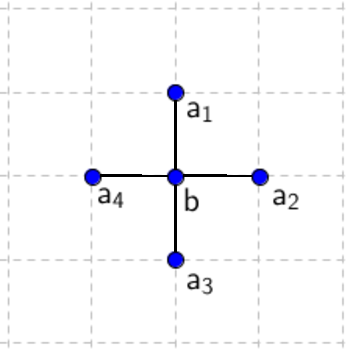
\includegraphics[width=3.5cm]{./img/disposicaoTortaGrid3}    
    & &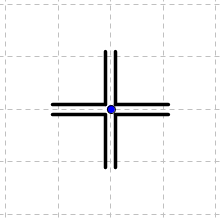
\includegraphics[width=3.5cm]{./img/truePieGrid} 
    & &
 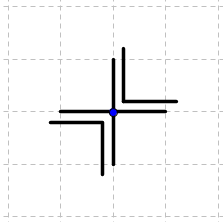
\includegraphics[width=3.5cm]{./img/falsePieGrid} \\%[\abovecaptionskip]
    {\footnotesize (a) 4-star in grid.}  & &  {\footnotesize (b) True pie.} & & {\footnotesize (c) False pie.} %\label{fig:frame}
  \end{tabular}
  \caption{$B_{1}$-EPG representation of the induced cycle of size 4 as pies with emphasis in center $b$.}\label{fig:piesInGrid2}
\end{figure} 


\begin{definition} \label{defi:tortasFrame2}
 Consider a rectangle of any size with 4 corners at points $ (x_1, y_1);$ $(x_2, y_1);$ $(x_2, y_2);$ $(x_1, y_2) $, positioned as in  Fig.~\ref{fig:frameInGrid}(a). 
 \begin{itemize}
 \item A \emph{frame} is a representation containing 4 paths $\mathcal{P} =  \{ P_1, \dots, P_4\} $, each having a bend in a different corner of a rectangle, and such that the  sub-paths $ P_1 \cap P_2, P_1 \cap P_3, P_2 \cap P_4, P_3 \cap P_4 $ share at least one edge. While $P_1 \cap P_4 $ and $ P_2 \cap P_3$ are empty sets.
 
 \item A square-frame is a frame where $P_1$, $P_2$, $P_3$ and $P_4$ have respectively point of bend $ (x_1, y_1),$ $(x_2, y_1),$ $(x_1, y_2)$ and $(x_2, y_2)$, and are of the shape $\llcorner$, $\lrcorner$, $\ulcorner$ and $\urcorner$.  (see Fig.\ref{fig:frameInGrid})
 \end{itemize}
\end{definition}

Fig.~\ref{fig:frameInGrid} illustrates some frame representations of a $C_4$.





\begin{figure}[htb]
  \centering
  \begin{tabular}{c c c c c }
    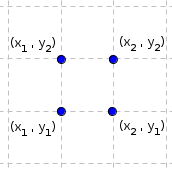
\includegraphics[width=3.5cm]{./img/dispositionFrameInGrid}    
    & &
   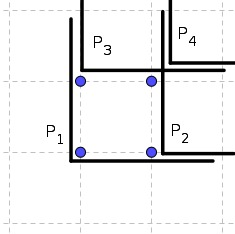
\includegraphics[width=3.5cm]{./img/frame2} 
     & &
   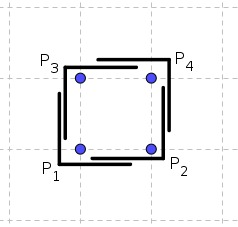
\includegraphics[width=3.5cm]{./img/square2} \\%[\abovecaptionskip]
   {\footnotesize (a) Coordinates of bends of a frame}  
   & & {\footnotesize (b) An example of a frame} 
   & & {\footnotesize (c) A square-frame} %\label{fig:frame}
  \end{tabular}
  \caption{$B_{1}$-EPG representation of the induced cycle of size 4 as frame}\label{fig:frameInGrid}
\end{figure} 


\begin{lemma}[\citet{golumbic2009}]\label{lem:representacaoC4}
Every  $C_4$ that is an induced subgraph of a graph $ G $ corresponds, in any representation, to a true pie, a false pie, or a frame.
\end{lemma}

The following is a claim of~\cite{heldt2014} which a reasoning can be found in~\cite{Asinowski2009}.

\begin{lemma}[\citet{daniel2014b} and \citet{Asinowski2009}]\label{fact:k24facts}
In every single bend representation of a $K_{2,4}$, the path representing each vertex of the largest part has its bend in a false pie.
\end{lemma} %fac

By creating four $K_{2,4}$ and identifying a vertex of the largest part of each one to a distinct vertex of a $C_4$, we construct the graph called bat graph (see Fig~\ref{fig:grafoQ}). Regarding to such a graph, the following holds.

\begin{figure}[htb]
  \centering
  \begin{tabular}{c c c c c }
    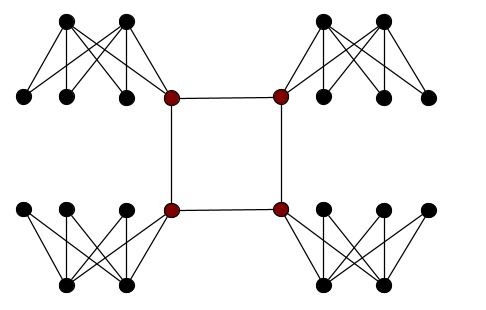
\includegraphics[width=5.5cm]{./img/Qexemplo}    
    & &
   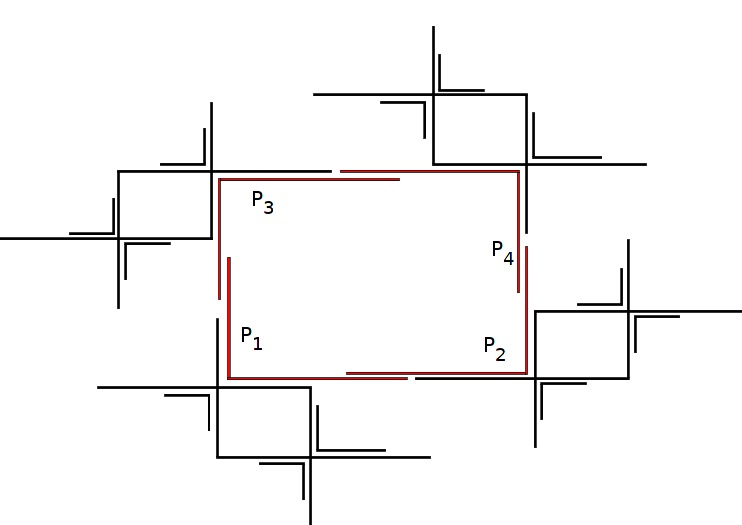
\includegraphics[width=8cm]{./img/representationQ}
  \end{tabular}
  \caption{A bat graph $G$ and a Helly-$B_1$-EPG representation of $G$.}\label{fig:grafoQ}
\end{figure} 

\begin{corollary}\label{batgraph}
In every single bend representation of the bat graph, $G$ presented in Fig.~\ref{fig:grafoQ}, the $C_4$ that is a transversal of all $K_{2,4}$ is represented by a square-frame.
\end{corollary}


\begin{figure}[htb]
  \centering
  \begin{tabular}{c c c c c }
   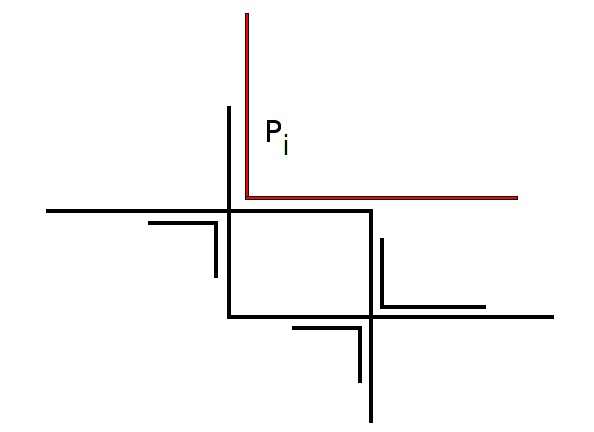
\includegraphics[width=5cm]{./img/representationQ2}
  \end{tabular}
  \caption{Helly-$B_1$-EPG representation of a $K_{2,4}$.}\label{fig:grafoQ2}
\end{figure} 

Figure~\ref{fig:grafoQ2} is an $B_1$-EPG representation for a $K_{2,4}$ graph. We know that any representation of a $K_{2,4}$ has the same shape for vertices in largest set, i.e. bending in a false pie. This fact is fundamental for the construction of a $B_1$-EPG representation of the bat graph, see Figure~\ref{batgraph}. When  we positioned a path $P_i$ corresponding to a vertex of the largest part of $K_{2,4}$ in construction of the bat graph, then we can state that the bend edge of each path $P_i$ does not be used by any non-member of this $K_{2,4}$. Thus each $P_i$ has to intersect another members of this $C_4$ by an extremity edge. Thus, we conclude that each path representing a vertex of the $C_4$ (transversal to all $K_{2,4}$) has its bend in a false pie and this $C_4$ is represented by a square-frame.

\begin{definition}
A $B_k$-EPG representation is \emph{minimal} 
when its set of edges does not properly contain another $B_k$-EPG representation. 
\end{definition}

The \textit{octahedral} graph is the graph containing 6 vertices and 12 edges, depicted  in Figure~\ref{fig:octaedro}(a). Next, we consider representations of the octahedral graph.
 

The next lemma follows directly from the discussion presented in~\cite{heldt2014}.

\begin{lemma}\label{lem:octaedronaohelly}
Every minimal $B_1$-EPG representation of the octahedral graph $O_3$ has the same shape.
\end{lemma}

 
\begin{figure}[h]
  \centering
  
%segundo bloco de figuras
  \begin{tabular}{@{}c@{} p{1.5cm} @{}c@{} }
   \centering 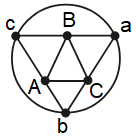
\includegraphics[width=2.5cm]{./img/octaedro.png} & &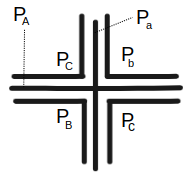
\includegraphics[width=4cm]{./img/representacaoOctaedro.png}  \\[\abovecaptionskip]
    \footnotesize \centering (a) O grafo octaedro $O_3$   & &  \footnotesize(b) Representação $B_1$-EPG do grafo $O_3$
  \end{tabular}

 \caption{O grafo octaedro $O_3$ e sua representação $B_1$-EPG}\label{fig:octaedro}
\end{figure}

The true pie presented in Figure~\ref{fig:octaedro}(b) is composite by paths corresponding to the vertex set $\{b, B, c, C\}$ of the Figure~\ref{fig:octaedro}(a). But in another $B_1$-EPG representation other paths corresponding to a different set of vertices could form the true pie, in any case, yet the shape is maintained. 



\section{Subclasses of $B_1$-EPG graphs}


By Lemma~\ref{lem:octaedronaohelly}, every minimal $B_1$-EPG representation of the octahedral graph $O_3$ has the same shape, as depicted in Fig.~\ref{fig:octaedro}(b). 
Since in any representation of the graph $O_3$ there is always a triple of paths that do not satisfy the Helly property, paths $P_{a}, P_{b} $ and $P_{c}$ in the case of Fig.~\ref{fig:octaedro}(b), it holds that $O_3 \notin$ Helly-$B_1$ EPG, which implies that the class of Helly-$B_1$-EPG graphs is a proper subclass of $B_1$-EPG.

Also, $B_0$-EPG and Helly-$B_0$-EPG graphs coincide. Hence, Helly-$B_0$ EPG can be recognized in polynomial time, see \cite{booth1976}.

%%%%%%%%%%%%%% 

In a $B_1$-EPG representation of a graph, the paths can be of the following four shapes: $\llcorner$, $\lrcorner$, $\ulcorner$ and $\urcorner$. \cite{cameron2016edge} studied $B_1$-EPG graphs whose paths on the grid belong to a proper subset of the four shapes. If $S$ is a subset of $\{\llcorner, \lrcorner, \ulcorner, \urcorner\}$, then $[S]$ denotes the class of graphs that can be represented by paths whose shapes belong to $S$, where zero-bend paths are considered to be degenerate $\llcorner$'s. They consider the natural subclasses of $B_1$-EPG: $[\llcorner], [\llcorner, \ulcorner], [\llcorner, \urcorner]$ and $[\llcorner, \ulcorner, \urcorner]$, all other subsets are isomorphic
to these up to 90 degree rotation. \cite{cameron2016edge}  showed that recognizing each of these classes is NP-complete.

The following shows how these classes relate to the class of Helly-$B_1$-EPG graphs.
%%%%%%%%%%%%%%

%\begin{figure}[htb]	
\center%6.3
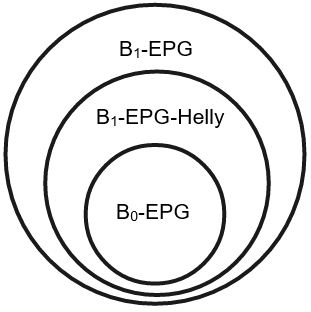
\includegraphics[width=3.5cm]{./img/diagramaClassesEPG.png}
\caption{Diagrama hierárquico de algumas classes  EPG}
\label{fig:diagramaEPG}
\end{figure}
\begin{figure}[H]	
\center%6.3
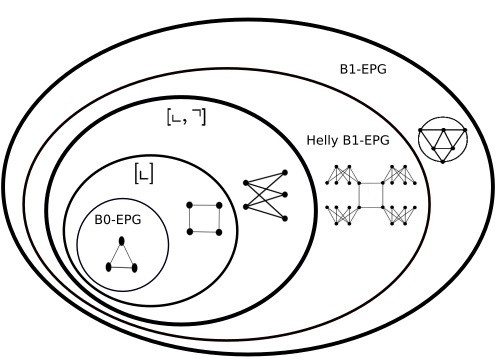
\includegraphics[width=8.5cm]{./img/classes} %2
\caption{Hierarchical diagram of some EPG classes}
\label{fig:diagramaEPG}
\end{figure}

\begin{theorem}\label{theo:HellyLShaped}
$[\llcorner]\subsetneq [\llcorner, \urcorner]\subsetneq$~Helly-$B_1$ EPG, and Helly-$B_1$ EPG is incomparable with $[\llcorner, \ulcorner]$ and $[\llcorner, \ulcorner, \urcorner]$.
\end{theorem}
\begin{proof}
\cite{cameron2016edge} showed that $[\llcorner]\subsetneq [\llcorner, \urcorner]$. Also, it is easy to see that $\llcorner$’s and $\urcorner$’s cannot form a claw-clique, thus, by Lemma~\ref{caracterization}, it follows that $[\llcorner, \urcorner]\subseteq$~Helly-$B_1$ EPG. In order to observe that $[\llcorner, \urcorner]$ is a proper subclass of Helly-$B_1$ EPG, it is enough to analyze the bat graph (see Fig.~\ref{fig:grafoQ}): by Corollary~\ref{batgraph} follows that any $B_1$-EPG representation of a bat graph contains a square-frame, thus it is not in $[\llcorner, \urcorner]$. In addition, the bat graph is bipartite which implies that any $B_1$-EPG representation of that graph does not contain claw-cliques and therefore is Helly.

Now, it remains to show that Helly-$B_1$ EPG is incomparable with $[\llcorner, \ulcorner]$ and $[\llcorner, \ulcorner, \urcorner]$. Again, since any $B_1$-EPG representation of a bat graph contains a square-frame, bat graph is a Helly-$B_1$-EPG graph that is not in $[\llcorner, \ulcorner, \urcorner]$. On the other hand, the $S_3$ (3-sun) is a graph in $[\llcorner, \ulcorner]$ such that any of its $B_1$-EPG representations have a claw-clique, see~Observation 7 in~\cite{cameron2016edge}. Therefore, $S_3$ is a graph in $[\llcorner, \ulcorner]$ that is not Helly-$B_1$ EPG.
\end{proof}

Figure~\ref{fig:diagramaEPG} depicts example of graphs of the classes $B_0$-EPG, $[\llcorner]$, $[\llcorner, \urcorner]$, Helly-$B_1$ EPG, and $B_1$-EPG that distinguish these classes.

It is known that recognizing $[\llcorner]$, $[\llcorner, \urcorner]$, and $B_1$-EPG are NP-complete while recognizing $B_0$-EPG and EPG graphs can be done in polynomial time (c.f.~\cite{booth1976}, \cite{heldt2014}, and \cite{cameron2016edge}).

Although the classes $ B_1$-EPG and Helly-$B_1$ EPG are distinct, the same is not true for the classes $B_0$-EPG and Helly-$B_0 $ EPG, because any $B_0$-EPG representation is Helly.  The $B_0$-EPG class corresponds exactly to class of interval graphs, see~\citet{booth1976}. Throughout the text we will show that each class of Helly-$B_k$ EPG is contained in the corresponding non-Helly class for all $ k \geq 1$, i.e. Helly-$B_k$ EPG $ \subsetneq$ $B_k$-EPG.

In this paper, we show that it is NP-complete to recognize Helly-$B_1$-EPG graphs.
%%%%%%%%%%%%%%%%%%%%%%%%%%%%%%%%%%%%%%%%%%%%%%%%%

\section{Membership in $\mathcal{NP}$} \label{sec:NPpert}

%In this paper we are interested in characterizing the complexity of the $B_1$-EPG-Helly recognition problem, whose formal definition is presented next:
Nesta seção, mostraremos que o problema de reconhecimento de grafos $B_k$-EPG-Helly, onde $k$ é limitado por um polinômio de $|V(G)|$, pertence a  $\mathcal{NP}$. O problema pode ser formalmente descrito como segue.

% \begin{table}[h!]
% \centering
% %\caption{My caption}
% %\label{my-label}
% \begin{tabular}{ll}
% \hline \hline
% \multicolumn{2}{c}{\sc Reconhecimento $B_k$-EPG-Helly}                         \\ \hline \hline 
% \emph{Entrada}: & Um grafo $G$, e um inteiro $k$.\\
%  & \\
% \emph{Objetivo}: & \begin{tabular}[c]{@{}p{12.5cm}}
% Determinar se existe um conjunto de caminhos $\mathcal{P} = \{P_1, P_2, \ldots, P_n\}$, com até $k$-dobras,  em uma grade  $ Q $ 
% tal que: \\
% \ \ $\bullet$ $v_i, v_j\in V(G)$ são adjacentes se e somente se  $P_i,P_j$ compartilham uma aresta em $Q$; \\
% \ \ $\bullet$ $\mathcal{P}$ satisfaz à propriedade Helly.
% \end{tabular} \\ \hline
% \end{tabular}
% \end{table}



\begin{table}[h!]
\centering
%\caption{My caption}
%\label{my-label}
\begin{tabular}{ll}
\hline \hline
\multicolumn{2}{c}{\sc Helly-$B_k$ EPG Recognition}                         \\ \hline \hline 
\emph{Input}: & A graph $G$ and an integer $k \leq |V(G)|^c$, for some fixed $c$.\\
~ & ~ \\
\emph{Goal:}  & \begin{tabular}[c]{@{}p{9.5cm}}
Determine if there is a set of $k$-bend paths \\ $\mathcal{P} = \{P_1, P_2, \ldots, P_n\} $ in a grid $ Q $ 
such that:\\ 
$\bullet$ \ \ \ $u,v\in V(G)$ are adjacent in $G$ if only if $P_u,P_v$\\ \hspace{0.6cm} share an edge in $Q$; and\\
$\bullet$ \ \ \ $\mathcal{P}$ satisfies the Helly property.
\end{tabular} \\ \hline
\end{tabular}
\end{table}


Um certificado (positivo) para o problema {\sc Reconhecimento $B_k$-EPG-Helly} consiste de uma grade $Q$, um conjunto de caminhos $\mathcal{P}$ com até $k$-dobras sobre $Q$, que tenham uma correspondência de um-para-um com os vértices do conjunto $V(G)$ de $G$, tais que, para cada par de caminhos distintos $P_i, P_j\in \mathcal{P}, P_i\cap P_j \neq \emptyset $  se e somente se os vértices correspondentes são adjacentes em $G$. Além disso, $\mathcal{P}$ deve satisfazer à propriedade Helly.

Os seguintes conceitos são centrais para nosso propósito.
Uma \emph{aresta relevante} em uma representação $B_k$-EPG é aquela que é aresta de extremidade ou uma aresta de dobra. Portanto, como cada caminho possui no máximo $k$ dobras, então cada caminho pode ter até $2(k+1)$ arestas relevantes, e qualquer representação $B_k$-EPG contém no máximo $2|\mathcal{P}|(k+1)$ arestas relevantes.

%O certificado para o algoritmo de verificação que mostra que um grafo é um grafo $B_k$-EPG-Helly possui como parâmetros de entrada uma representação $B_k$-EPG, chamemos de $R$, contendo uma coleção de caminhos $\mathcal{P}$, $|\mathcal{P}|=|V(G)|$, onde cada caminho  $P_i \in \mathcal{P}$ é dado pelo seu conjunto de arestas relevantes mais o conjunto de arestas relevantes, que intersectam   $P_i$, de outros caminhos. As arestas relevantes devem ser dadas na ordem em que aparecem no caminho. Esse formato de codificação para os caminhos nos permite verificar se cada conjunto de arestas relevantes realmente representa um caminho com no máximo $k$-dobras. Essa representação também é útil para verificar se as intersecções correspondem a um modelo de intersecção para $G$.

%Um certificado (positivo) para  {\sc Reconhecimento $B_k$-EPG-Helly} consiste de uma grade $Q$, um conjunto  $\mathcal{P}$ de caminhos com $k$-dobras sobre $Q$, which have a one-to-one correspondence with the vertex set $V(G)$ of $G$, such that, for each pair of distinct paths $P_i, P_j\in \mathcal{P}, P_i\cap P_j \neq \emptyset $ if and only if the corresponding vertices are adjacent in $G$. Furthermore, $\mathcal{P}$ satisfies the Helly property.


Para mostrar que existe um algoritmo de tempo polinomial não determinístico para {\sc Reconhecimento $B_k$-EPG-Helly}, é suficiente considerar como certificado uma representação $B_k$-EPG, digamos  $R$, contendo uma coleção de caminhos  $\mathcal{P}$, onde $|\mathcal{P}| = |V(G)|$, tal que cada caminho   $P_i \in \mathcal{P}$  é dado pelo seu conjunto de arestas relevantes juntamente com o conjunto de todas as arestas relevantes de $P_j$ que intersectam $P_i$, onde $P_j \in \mathcal{P}$.  % as arestas relevantes, que intersectam $P_i$, de cada caminho $P_j$ que intersecta  $P_i$, onde $P_j \in \mathcal{P}$. 
 As arestas relevantes para cada caminho são dadas na ordem em que elas aparecem no caminho, de forma que é fácil checar se as arestas correspondem a um caminho único com no máximo  $k$ dobras. Essa representação é também utilizada para checar se os caminhos formam um modelo de intersecção para  $G$.

A fim de verificar, em tempo polinomial, que a entrada de fato é um certificado para o problema, temos que verificar as seguintes afirmações:

\begin{enumerate}[label=(\roman*)]
\item A sequência de arestas relevantes de um caminho $P_i\in \mathcal{P}$ determina unicamente $P_i$ em tempo polinomial; \label{it:bullet1}

\item Dois caminhos  $P_i, P_j \in \mathcal{P}$ são intersectantes se e somente se eles se intersectam em alguma aresta relevante; \label{it:bullet2}

\item O conjunto  $\mathcal{P}$ de arestas relevantes satisfaz à propriedade Helly. \label{it:bullet3}
\end{enumerate}

O Lema a seguir mostra que a condição~\ref{it:bullet1} é válida.

\begin{lema}\label{lem:verify1}
Cada caminho $P_i$ pode ser determinado unicamente, em tempo polinomial pela sua sequência de arestas relevantes.
\end{lema}

\begin{proof}
É fácil verificar que o item~\ref{it:bullet1} é verdadeiro. Considere a sequência de arestas relevantes de algum caminho $P_i\in \mathcal{P}$. Inicie de uma aresta de extremidade de $P_i$. Seja   $t$ a linha (coluna) contendo a última aresta relevante considerada. A próxima aresta relevante  $e'$ na sequência, deve estar contida na linha (coluna) $t$. Se $e'$ é uma aresta de extremidade, o processo está terminado e o caminho terá sido determinado. Ele contém todas arestas entre as arestas relevantes consideradas na sequência.  Caso contrário, se  $e'$ é uma aresta de dobra, a próxima aresta relevante é é a segunda aresta de dobra  $e''$ da mesma dobra, que está contida em alguma coluna (linha) $t'$. O processo continua até que a segunda aresta de extremidade de $P_i$ estar localizada.   

Com o procedimento acima podemos determinar em tempo $\mathcal{O}(k\cdot |V(G)|)$, se o caminho $P_i$ contém qualquer dada aresta da grade $Q$. Além disso, a sequência de arestas relevantes de  $P_i$ determina unicamente  $P_i$.
 \end{proof} %$\square$

O lema abaixo mostra que o item~\ref{it:bullet2} é válido.

\begin{lema}\label{lem:relevantEdges}
Seja $\mathcal{P}$ o conjunto de caminhos em uma representação $B_k$-EPG $R$ de $G$, e sejam $P_1,P_2 \in \mathcal{P}$. Então $P_1, P_2$ são caminhos intersectantes se e somente se sua intersecção contém no mínimo uma aresta relevante.%eles contêm no mínimo uma aresta relevante em comum.
\end{lema}

\begin{proof}
Se $P_1, P_2$ contém uma aresta relevante comum então claramente eles são intersectantes. Caso contrário, considere que $P_1, P_2$ são intersectantes, e mostraremos que eles contêm uma aresta relevante comum. Sem perda de generalidade, suponha que $P_1, P_2$ intersectam-se na linha \textit{i} da grade, em uma representação   $B_k$-EPG, digamos $R$. As seguintes são as possibilidades que podem ocorrer. 

Seja $e$ uma aresta comum a $P_1$ e $P_2$. Se $e$ não é aresta relevante, então a aresta seguinte à  esquerda (ou direita) de $e$, digamos $e'$, também pertence a $P_1 \cap P_2$. Tome $e'$, se $e'$ é relevante, então encontramos a aresta relevante da intersecção de $P_1$ e $P_2$, se não repetimos o processo até que uma aresta relevante seja encontrada. Caso os caminhos sejam juntos, uma aresta de dobra ou de extremidade é comum aos dois. Caso os dois caminhos se separem em algum ponto também existe uma aresta de dobra ou de extremidade que é comum aos dois.

% \begin{itemize}
% \item \textbf{Caso 1:} Nem $P_1$ nem $P_2$ contêm dobras na linha \textit{i}. 

% Então $P_1$ e $ P_2$  estão inteiramente contidos na linha \textit{i}. Uma vez que eles se intersectam, ou  $P_1, P_2$  se cobrem parcialmente, ou um dos caminhos contém o outro. Em qualquer dessas situações eles intersectam em uma aresta de extremidade comum, que é uma aresta relevante.

% \item \textbf{Caso 2:} $P_1$ não contém dobras em \textit{i}, mas $ P_2$ contém.

% Se alguma aresta de dobra de $P_2$ também pertence a   $P_1$, então $P_1, P_2$  intersectam-se em uma aresta relevante. Caso contrário, uma vez que $P_1, P_2$  intersectam-se, a única possibilidade é que a intersecção contenha uma aresta de extremidade de  $P_1$ ou $ P_2$. Portanto, os caminhos se intersectam em uma aresta relevante.

% \item \textbf{Caso 3:} Ambos $P_1$,  $P_2$ contém em \textit{i}.

% Novamente, se a intersecção ocorre em alguma aresta de dobra de $P_1$  ou $P_2$, o lema segue válido. Caso contrário,  a mesma situação anterior deve ocorrer, ou seja, $P_1, P_2$  devem intersectar em alguma aresta de extremidade.
 
% \end{itemize}
Em qualquer dos casos, $P_1$ e $P_2$ intersectam-se em alguma aresta relevante.
\end{proof}

Os dois lemas anteriores nos permitem checar que um certificado é uma representação $B_k$-EPG correta de um dado grafo $G$. O próximo lema diz que podemos verificar em tempo polinomial que a representação codificada em um certificado é uma representação Helly. Felizmente nós não precisamos checar todos os subconjuntos de caminhos intersectantes da representação para ter certeza que eles possuem uma intersecção comum.

Finalmente, provamos o item~\ref{it:bullet3}.


\begin{lema}\label{lem:verify3}
Seja $\mathcal{P}$ uma coleção de caminhos codificados como uma sequência de arestas relevantes que constituem uma representação $B_k$-EPG  de um grafo  $G$. Podemos verificar em tempo polinomial se $\mathcal{P}$  possui a propriedade Helly.
\end{lema}


\begin{proof}
Seja $\mathcal{T}$ o conjunto de arestas relevantes de $\mathcal{P}$. Consideramos cada tripla $T_i$ de arestas de  $\mathcal{T}$. Seja $\mathcal{P}_i$ o conjunto de caminhos de  $\mathcal{P}$ contendo no mínimo duas arestas relevantes de $T_i$. Pelo Teorema de Gilmore~\cite{bergeDuchet1975}, $\mathcal{P}$ possui a propriedade Helly se e somente se o subconjunto de caminhos de $\mathcal{P}_i$ correspondendo a cada tripla de $T_i$ tem intersecção não vazia.  Pelo Lema~\ref{lem:relevantEdges} é suficiente examinar a intersecção das arestas relevantes.  Além disso, um algoritmo polinomial para checar se $\mathcal{P}$ possui a propriedade Helly poderia examinar cada um dos subconjuntos $P_i$, e para cada aresta relevante $e$ de um caminho em $P_i$, computar o número de caminhos em $P_i$ que contêm $e$. $\mathcal{P}$ tem a propriedade Helly se e somente se para cada $P_i$ existe alguma aresta relevante que está em todos os caminhos de $P_i$ produzindo uma intersecção não vazia.
 \end{proof} %$\square$


\begin{corollary}\label{cor:comumAtodos}
Seja ${\mathcal P'}$ um conjunto mutuamente intersectante de caminhos em uma representação $B_k$-EPG-Helly de um grafo  $G$. Então a intersecção de todos os caminhos de ${\mathcal P'}$ contém no mínimo uma aresta relevante.
\end{corollary}

Note que a propriedade descrita no Corolário~\ref{cor:comumAtodos} é devida ao Teorema de Gilmore~\cite{bergeDuchet1975}, e se aplica somente a representações que satisfazem à propriedade Helly.

\medskip


\begin{lemma}\label{lem:gridPolinomial}
Seja $G$ um grafo $B_k$-EPG-Helly. Então $G$ admite uma representação $B_k$-EPG-Helly sobre uma grade de tamanho que é no máximo $4n(k+1) \times 4n(k+1)$.
\end{lemma}
\begin{proof}
Seja $R$ uma representação $B_k$-EPG de um grafo $G$ sobre uma grade $Q$ com o menor tamanho possível.
Seja $\mathcal{P}$ o conjunto de caminhos de  $R$. Note que $|\mathcal{P}|=n$.
 Existem no máximo $2|\mathcal{P}|(k+1)$ arestas relevantes em  $R$. 
 Se $Q$ possui um par de colunas consecutivas $c_i,c_{i+1}$ que não contém arestas relevantes de  $R$, e tais que não existem arestas relevantes cruzando de $c_i$ para $c_{i+1}$, então podemos contrair cada aresta cruzando de $c_i$ para $c_{i+1}$ em um único vértice de forma a obter uma nova representação  $B_k$-EPG  $G$ sobre uma grade de menor tamanho, o que é uma contradição. Um argumento análogo pode ser aplicado a pares de linhas consecutivas da grade.
  Portanto, a grade  $Q$ é tal que cada par de colunas consecutivas e de linhas consecutivas de  $Q$ tem no mínimo uma aresta relevante de $R$ ou contém uma aresta relevante cruzando-as.  
  Como $Q$ é a menor grade possível para representar  $G$ então a primeira linha e a primeira coluna de $Q$ ambas devem conter no mínimo um ponto  pertencendo a alguma aresta relevante de $R$. 
Assim, se $G$ é $B_k$-EPG então ele admite uma  representação $B_k$-EPG sobre uma grade de tamanho no máximo $4|\mathcal{P}|(k+1) \times 4|\mathcal{P}|(k+1)$.
Além do mais, pelo  Corolário~\ref{cor:comumAtodos}, sustenta-se que a operação de contração anteriormente descrita preserva à propriedade Helly, se houver. Assim, sendo $R$ uma representação $B_k$-EPG-Helly de um grafo $G$ sobre uma grade $Q$ com tamanho mínimo possível, é seguro afirmar que $Q$ possui tamanho no máximo  $4|\mathcal{P}|(k+1) \times 4|\mathcal{P}|(k+1)$.
\end{proof}

\begin{theorem}\label{teo:nppertinencia}
{\sc Reconhecimento $B_k$-EPG-Helly} está em  $\mathcal{NP}$, sempre que $k$ é limitado por uma função polinomial de $|V(G)|$.
\end{theorem}
\begin{proof}
Pelo Lema~\ref{lem:gridPolinomial} e o fato de que $k$ é limitado por uma função polinomial de  $|V(G)|$, segue que a coleção  $\mathcal{P}$ pode ser codificada através de suas arestas relevantes com   $n^{\mathcal{O}(1)}$ bits.

Finalmente, pelos Lemas~\ref{lem:verify1}, \ref{lem:relevantEdges} e \ref{lem:verify3}, segue que podemos verificar em tempo polinomial sobre o tamanho de $G$ se $\mathcal{P}$ é uma família de conjuntos codificada como uma sequência de arestas relevantes que constituem uma representação $B_k$-EPG-Helly de um grafo  $G$.
\end{proof}

\section{$NP$-Hardness}\label{sec:sectionDispositivoClausula}

Agora provaremos que o reconhecimento de grafos   $B_1$-EPG-Helly é $NP$-completo. Para essa demonstração seguiremos o roteiro de prova de dificuldade traçado por~\cite{heldt2014}.  Estabelecemos a redução do problema {\sc Positive (1 in 3)-3SAT} definido como segue:

\begin{table}[h!]
\centering
%\caption{My caption}
%\label{my-label}
\begin{tabular}{ll}
\hline \hline
\multicolumn{2}{c}{\sc Positive (1 in 3)-3SAT}                                \\ \hline \hline 
\emph{Entrada}: & \begin{tabular}[c]{@{}p{12.5cm}@{}} Um conjunto $X$ de variáveis positivas; uma coleção $\mathcal{C}=\{C_1,C_2,\ldots,C_m\}$ de cláusulas sobre  $X$ tal que para cada $C_i\in \mathcal{C}$, $|C_i|= 3$.
\end{tabular} \\
 &  \\
\emph{Objetivo}:  & \begin{tabular}[c]{@{}l@{}} %@{}l@{}
Determinar se existe uma atribuição de valores para as variáveis em $ X $\\ de modo que toda cláusula em  $\mathcal{C}$ tem exatamente um literal verdadeiro.
\end{tabular} \\ \hline
\end{tabular}
\end{table}

{\sc Positive (1 in 3)-3SAT } é um problema $NP$-completo bem conhecido (ver \cite{johnson1979}, problema [L04], pág. 259). {\sc Positive (1 in 3)-3SAT} permanece $NP$-completo quando o grafo de incidência da fórmula CNF (Conjunctive Normal Form) é um grafo planar~\cite{mulzer2008minimum}.

Dada uma fórmula  $F$ que é uma instância de {\sc Positive (1 in 3)-3SAT} apresentaremos uma construção de tempo polinomial de um grafo $ G_F$ tal que  $ G_F $ é $ B_1$-EPG-Helly se e somente se $ F $ é satisfativa. Esse grafo conterá um subgrafo induzido  $ G_{c_i}$ com 12 vértices (chamado \emph {dispositivo cláusula}) para toda cláusula $C_i \in F$, e um subgrafo induzido (\emph {dispositivo variável}) para cada variável $ x_j$, contendo um vértice especial   $ v_j$, além de um  \emph{dispositivo base}  com 55 vértices adicionais.

%Since a Sun graph $S_4$ whose centro is a cycle of size 4 and adding a false twin to each vertex of $S_4$ that is not a member of central induced cycle then we have the graph $H$. 
Utilizaremos um grafo $H$ isomorfo ao grafo ilustrado na Figura~\ref{fig:gadgetBase}, como um  dispositivo para realizar a prova. Para cada cláusula  $C_i$ de $F$ do nosso problema alvo, teremos um \emph{dispositivo cláusula} isomorfo a $H$, denotado por $G_{C_i}$. %The graph $H$ consists of subgraphs whose $B_1$-EPG representations are well known, such as: cycles of sizes 3 and 4.

\begin{figure}[htb]	
\center%6.3
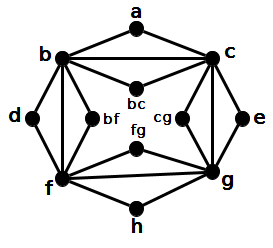
\includegraphics[width=5cm]{./img/gadgetBase.png}
\caption{The partial gadget graph $H$.}
\label{fig:gadgetBase}
\end{figure} 

%\subsection{Definition}\label{sec:reducao}%The problem reduction}

A redução  de uma instância $F$ de  {\sc Positive (1 in 3)-3SAT}  para um grafo particular $G_F$ tal que $G_F$ possui uma representação $B_{1}$-EPG-Helly se e somente se $F$ é satisfatível, é dada abaixo.

\begin{definition}\label{sec:reducao}
Seja $F$ uma fórmula na CNF sem literais negativos, em que toda cláusula possui exatamente três literais. O grafo $G_F$ é construído como segue:

\begin{enumerate}
\item Para cada cláusula $C_i \in F$ criar um \textit{dispositivo cláusula} $G_{C_i}$, isomorfo ao grafo $H$;

\item Para cada variável $x_{j}$ criar um \emph{vértice-variável} $v_{j}$ que é adjacente aos vértices $a$, $e,$ ou $h$ de $G_{C_i}$, quando $x_{j}$ é a primeira, segunda ou terceira variável em $C_i$, respectivamente;

\item Para cada vértice-variável $v_{j}$, construir um \emph{dispositivo variável} formado pela adição de duas cópias de  $H$, digamos $H_1$ e $H_2$, e fazendo $v_j$ adjacente aos vértices do triângulo $(a, b, c)$ em  $H_1$ e $H_2$.

 %where $v_{j}$ is  adjacent to all vertices of the triangle (a,b,c);%; (c,e,g); (g,f,h); or (b,d,f)) of each $H_1$ and $H_2$; 

%\item The  subgraph induced by \emph{vértice-variável}  $v_{j}$, and also $V(H_1)$ and $V(H_2)$ will be called \emph{dispositivo variável}; 

\item Criar um vértice $V$, que será utilizado como referência vertical para a construção, e adicionar arestas de  $V$ para cada vértice  $d$ nos \emph{dispositivos cláusula};%$d \in V(G_c)$;

\item Criar um grafo bipartido $K_{2,4}$ com um vértice particular $T$ que faz parte do maior conjunto estável desse $K_{2,4}$. Esse vértice é denominado \emph{vértice-verdadeiro}. $T$ é adjacente a todos  $v_{j}$ e também a $V$;

\item Criar dois grafos isomorfos a $H$, digamos $G_{B1}$ e $G_{B2}$. O vértice $T$ é conectado a todos os vértices do triângulo $(a,b,c)$
em $G_{B1}$ e $G_{B2}$;


\item Criar dois grafos isomorfos a $H$, digamos $G_{B3}$ e $G_{B4}$. O vértice $V$ está conectado a todos os vértices do triângulo $(a,b,c)$ em $G_{B3}$ e $G_{B4}$;

\item O subgrafo induzido pelo conjunto de vértices $\{V(K_{2,4}) \cup  \{T, V\} \cup V(G_{B1}) \cup V(G_{B2}) \cup V(G_{B3}) \cup V(G_{B4})\}$ será denominado como \emph{dispositivo base}. 
\end{enumerate}
\end{definition}


A Figura~\ref{fig:exemploGrafoGF} retrata como essa construção funciona quando aplicada sobre uma pequena fórmula. %represents the graph that would be obtained when the previous construction is applied to the formula $ F = (x_1 + x_2 + x_3) \wedge (x_2 + x_3 + x_4) \wedge (x_3 + x_1 + x_4)$.


\begin{figure}[htb]	
\center%6.3
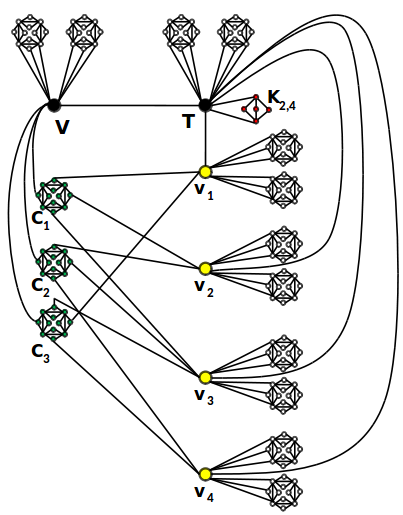
\includegraphics[width=6.5cm]{./img/exemploGrafoGFSBPO4.png}
\caption{O grafo $G_{F}$ correspondendo à fórmula $F=(x_1+ x_2+ x_3) \wedge  (x_2+ x_3+ x_4 )\wedge  (x_3 + x_1 + x_4 )$}
\label{fig:exemploGrafoGF}
\end{figure}


\begin{lema}\label{lem:ida}
Dada uma instância satisfatível $F$ de {\sc Positive (1 in 3)-3SAT}, o grafo  $G_F$ construído a partir de $F$ de acordo com a Definição~\ref{sec:reducao} admite uma representação $B_{1}$-EPG-Helly.
\end{lema}


\begin{proof}

%~\ref{fig:representacaoCaminhos}
Utilizaremos as estruturas  torta verdadeira e torta falsa para representar os  \textit{dispositivo cláusula} $ G_C$, mas a construção poderia ser feita com a estrutura moldura sem perda de generalidade, ver Figura~\ref{fig:falseAndTruePie}.  


\begin{figure}[htb]
  \centering
%segundo bloco de figuras
  \begin{tabular}{c c c }
    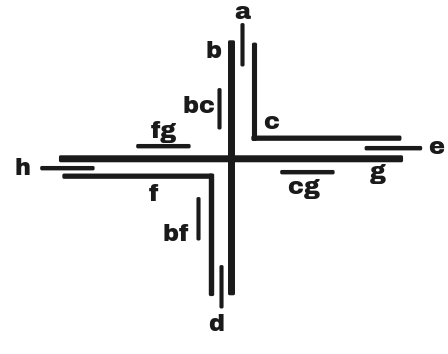
\includegraphics[width=4.5cm]{./img/falsePie.png}  %\label{fig:falsePie} 
    & &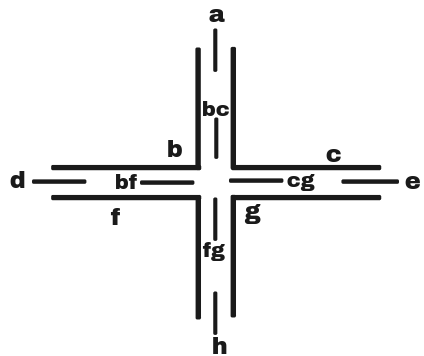
\includegraphics[width=4.5cm]{./img/truePie.png} %\label{fig:truePie}
    \\%[\abovecaptionskip]
    {\footnotesize (a) Baseado em torta falsa}  & &  {\footnotesize(b) Baseado em torta verdadeira}\\
  \end{tabular}
  \caption{Representação de dobra simples  de um dispositivo cláusula isomorfo ao grafo $H$} \label{fig:falseAndTruePie}
\end{figure} 

Os \textit{dispositivo variável} serão representados por estruturas como da Figura~\ref{fig:gadgetVariavel}.

\begin{figure}[htb]	
\center%6.3
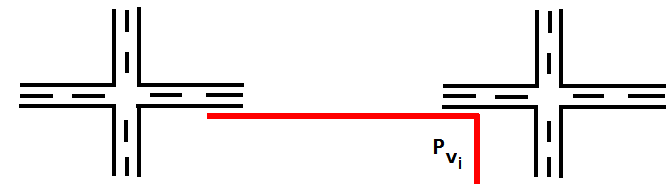
\includegraphics[width=10cm]{./img/gadgetVariavel.png}
%clausulaGadgetGFCompletaSBPO
\caption{Representação de dobra simples de um dispositivo variável}
\label{fig:gadgetVariavel}
\end{figure}


O \textit{dispositivo base} será representado pela estrutura retratada na  Figura~\ref{fig:gadgetBaseSingleBend}.

\begin{figure}[htb]	
\center%6.3
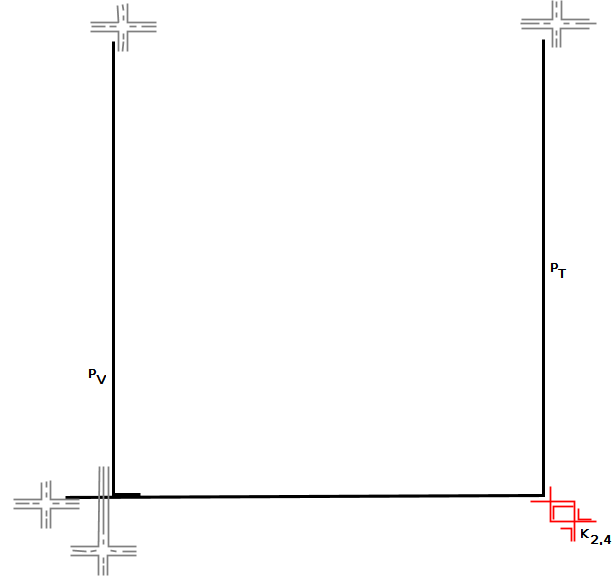
\includegraphics[width=10cm]{./img/gf2.png}
%clausulaGadgetGFCompletaSBPO
\caption{Representação de dobra simples do dispositivo base}
\label{fig:gadgetBaseSingleBend}
\end{figure}


É fácil ver que as representações dos dispositivo cláusula, dispositivo variável e dispositivo base são todas  $B_1$-EPG-Helly. Agora precisamos descrever como essas representações podem ser combinadas de forma a construir uma representação  de dobra simples $R_{G_F}$.

Dada uma atribuição  $A$ que satisfaz  $F$, podemos construir uma representação $R_{G_F}$ que seja  $B_{1}$-EPG-Helly. Primeiro, fixaremos a estrutura de representação do dispositivo base na grade para organizar a representação, ver Figura~\ref{fig:gadgetBaseSingleBend}. A seguir inserimos o  dispositivo variável com a seguinte regra: se a variável $x_i$ relacionada ao caminho   $P_{v_i}$ tiver atribuição  \textit{True}, então a adjacência entre o caminho $P_{v_i}$ com $P_{T}$ é horizontal, e vertical caso contrário. Por exemplo, uma atribuição  $A=\{x_1=False; x_2=False;x_3=True; x_4=False\}$  para as variáveis da fórmula  $F$ que gerou o dispositivo $G_F$ da Figura~\ref{fig:exemploGrafoGF}, nos dará um representação de dobra simples (dispositivo base + dispositivo variável) de acordo com a  Figura~\ref{fig:gadgetBasePlusVariables}(a). 

Quando a fórmula  $F$ de {\sc Positive (1-in-3)-3sat} possui cláusulas cujo formato de atribuição é $(False, True, False)$ ou $(False, False, True)$ então usaremos torta falsa para representar essas cláusulas, mas quando a cláusula tem formato  $(True, False, False)$ utilizaremos  torta verdadeira para representar essa cláusula. Para inserir um  \textit{ dispositivo cláusula} $G_{C_i}$, introduziremos uma linha horizontal $l_{h}$ na grade entre as linhas horizontais usadas pelos caminhos para as duas variáveis $False$ em $ C_i $. Então conectaremos o caminho $P_{d_{c_i}}$ de $G_{C_i}$ em $P_{V}$ verticalmente usando a dobra de  $P_{d_{c_i}}$. No entanto, introduziremos uma linha vertical $ l_{v}$, na grade, entre a linha vertical da grade usada por $P_{V}$ e o caminho para  a variável $True$ em $C_i$, i.e. entre $P_{V}$ e o caminho representando a variável  $x_j \in C_i$. Onde  $l_{h}$  e $l_{v}$ cruzarem, nesse ponto iremos inserir o centro do  \textit{dispositivo cláusula} como pode ser visto na Figura~\ref{fig:gadgetOnePie}(b). Uma construção completa dessa representação de dobra simples para  $G_F$ pode ser verificada na 
Figura~\ref{fig:gadgetFormulaCompletaPies}.%~\ref{fig:clausulagadgetgf}. 

\begin{landscape}
\begin{figure}[h]
  \centering
%segundo bloco de figuras
  \begin{tabular}{p{10cm} p{2cm} p{10cm}}
   \centering 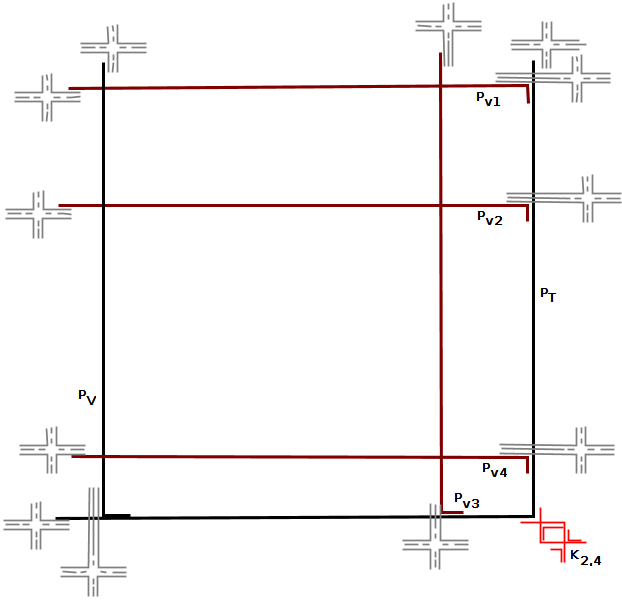
\includegraphics[width=10cm, left]{./img/gf3.png} & & 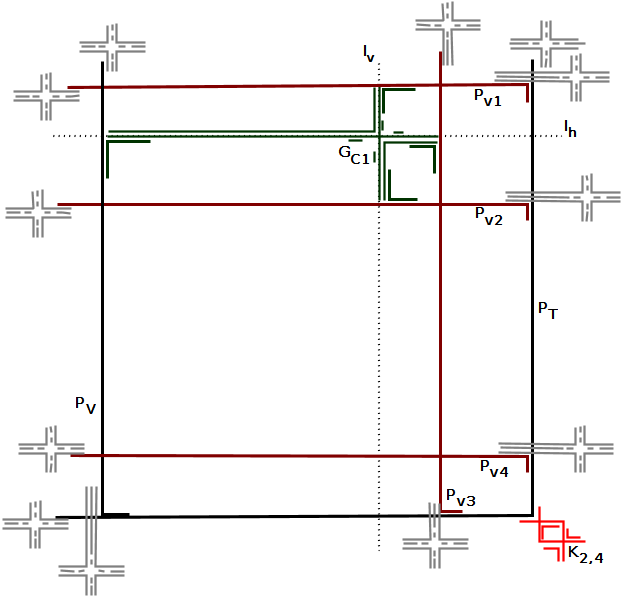
\includegraphics[width=10cm, left]{./img/formulaCompletaGFonePiePlusLines.png} \\  
  [\abovecaptionskip]
    \footnotesize \centering (a) Representação com dispositivos cláusula omitidos & & \footnotesize(b) Representação  com  $G_{C_1}$  associado com a cláusula $(x_1+x_2+x_3)$ em destaque \\
  \end{tabular}

 \caption{Representação de dobra simples dos dispositivos base e variáveis associados com as atribuições $x_1=False, x_2=False, x_3=True, x_4=False$} \label{fig:gadgetOnePie} \label{fig:gadgetBasePlusVariables}
\end{figure}
\end{landscape}


\begin{figure}[htb]	
\center%6.3
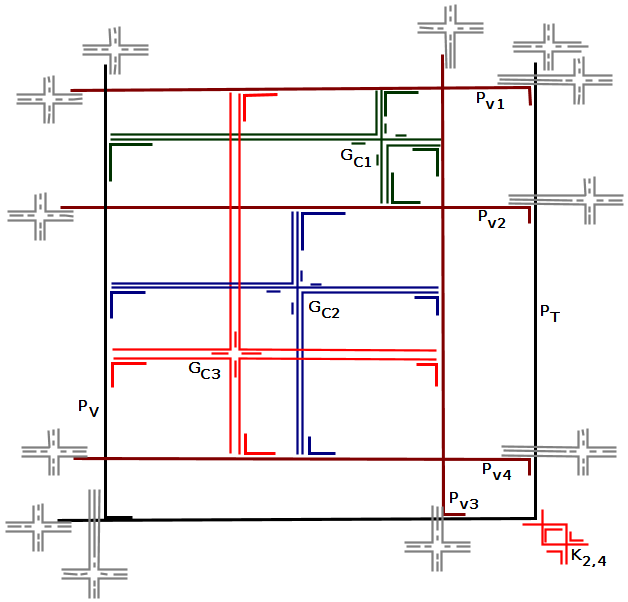
\includegraphics[width=10cm]{./img/formulaFGCompletaPies.png}
%clausulaGadgetGFCompletaSBPO
\caption{Representação de dobra simples de $G_F$}
\label{fig:gadgetFormulaCompletaPies}
\end{figure}


Note que quando juntamos todas essas representações  dos  dispositivos que formam $ R_{G_F} $ não há inserção de mais dobras nos caminhos que já possuíam dobra, então a representação necessariamente permanece sendo uma representação  $ B_1$-EPG válida. Nos resta mostrar que ela satisfaz à propriedade Helly. 

Uma forma simples de verificar que $ R_{G_F} $ satisfaz à propriedade Helly é notar que o grafo particular  $G_F$ nunca forma triângulos entre dispositivo variável, cláusula e base. Assim, qualquer triângulo de  $G_F$ está contido nos dispositivo variável, cláusula ou base. Como usamos somente representações  $B_1$-EPG-Helly desses dispositivos, $ R_{G_F} $ permanece uma representação $B_1$-EPG-Helly de $G_F$.
 \end{proof}

%\cleardoublepage
%\newpage

A seguir consideramos a conversão. Tome uma representação $B_1$-EPG-Helly, $R$ de $G_F$.

%To complete the proof of $NP$-hardness we will  present some considerations related with the single bend representation of gadgets that form the graph $G_F$. The way all gadgets can be drawn makes it possible to recover the formula that generated $G_F$ and a $True-$assignment for it. The following proofs help us understand the construction of a representation to $G_F$.  

\begin{definition}
Seja $H$ o grafo mostrado na  Figura~\ref{fig:gadgetBase}, tal que um 4-ciclo $H[\{b, c, f, g \}]$ corresponde em $R$ a uma estrutura de torta falsa ou torta verdadeira, então:

\begin{itemize}
\item O \emph{centro} é o único ponto da grade dessa representação que está contido em todo caminho representando o 4-ciclo $ \{b, c, f, g \}$; \label{lab:lab1}

\item Um \emph {raio central} é uma aresta-intersecção entre dois dos caminhos correspondendo aos vértices $ b, c, f, g$, respectivamente.
\end{itemize}
\end{definition}


Note que toda representação $B_1$-EPG de um $C_4$ satisfaz à propriedade Helly, ver Lema~\ref{lem:representacaoC4}, e os triângulos possuem $B_1$-EPG representações que satisfazem à propriedade Helly, e.g. a retratada na Figura~\ref{fig:trianguloepgRepresentacao}(b). O grafo $H$ é composto por um 4-ciclo,  $C_4^{H}=H[b, c, f, g]$ e oito triângulos, que são $(a,b,c);$ $(b,c,bc);$ $(c,e,g);$ $(c,g,cg);$ $(f,g,h);$ $(f,g,fg);$ $(b,d,f);$ $(b,f,bf).$

Como $C_4^{H}$ é um grafo que possui representações bem conhecidas (ver Lema~\ref{lem:representacaoC4}), então podemos iniciar o desenho da representação $B_{1}$-EPG-Helly de $H$ dessas estruturas. As  Figuras~\ref{fig:falsepietruepieframe} retratam possibilidades de representações para $H$.

Se um $C_4^{H}$ é representado por torta verdadeira ou torta falsa, então os caminhos $P_b, P_c, P_f, P_g$ compartilham um ponto central da representação. Por outro lado, se  $C_4^{H}$ é representado por uma moldura então as dobras dos caminhos correspondem aos quatro cantos distintos de um retângulo, i.e. todos os caminhos representando  vértices de um $C_4^{H}$ possuem pontos de dobra distintos, ver~\cite{golumbic2009}.

A seguir examinaremos o uso da estrutura moldura.

%Due asymmetric representations, the moldura structure needs to be studied in more detail. Next we will show some constraints of this structure. % in which allow us to consider it. %as gadget in the demonstration.

\begin{proposition}\label{lem:direcoesdiferentes}
Em uma representação $B_1$-EPG de um $C_4$ isomorfa a uma moldura, todo caminho  $P_i$ que representa um vértice do $C_4$ intersecta exatamente dois outros caminhos $P_{i-1}$ e $P_{i+1}$ da moldura, de modo que uma das intersecções é vertical e a outra é horizontal. %where one of them is vertical and another is a horizontal intersection.
\end{proposition}

\begin{proof}
A prova é imediata, pela definição de moldura.
 \end{proof}

\begin{proposition}\label{lem:mesmaretasuporte}
Dada uma representação $B_1$-EPG-Helly de um grafo $G$ que possui um $C_4$ induzido cuja representação é isomorfa a uma moldura. Se existe um vértice $v$ de $G$, fora desse $C_4$, que é adjacente a exatamente dois vértices consecutivos desse $C_4$, então o caminho representado por  $v$ possui uma aresta comum com os caminhos representando ambos vértices do $C_4$.% of $v$ into such .  
\end{proposition}

\begin{proof}
Por suposição, $G$ possui um triângulo contendo  $v$ e dois vértices de um $C_4$ representado por moldura. Além disso, o caminho representando  $v$ compartilha no mínimo uma aresta que é intersectante aos caminhos que representam seus vizinhos, caso contrário a representação não satisfaz à propriedade Helly.
 \end{proof}

%\cleardoublepage

Pela Proposição~\ref{lem:direcoesdiferentes} e Proposição~\ref{lem:mesmaretasuporte} podemos concluir que para todo vértice   $v_i \in V(H)$ tal que $v_i \neq V(C_4^{H})$, quando usamos uma moldura para representar o $C_4^{H}$, $P_{v_i}$ terá no mínimo uma aresta-intersecção comum ao par de caminhos representando seus vértices vizinhos em $H$. 
A Figura~\ref{fig:falsepietruepieframe}(c) retrata uma possível representação $B_{1}$-EPG-Helly de $H$. 
Note que ao aplicarmos operações de rotação e espelhamento, mantemos a representação $B_1$-EPG-Helly de $H$.
%On this $B_{1}$-EPG-Helly representation presented we can apply rotation and mirroring operations, because these operations do not change the structure. We can also a change the direction of the bend (see Figure~\ref{fig:falsepietruepieframe}(c) and Figure~\ref{fig:outraRepresentacaoFrame}), but also adjust other paths if needed, so as to not change the intersections between the paths.

\begin{definition}
Em uma representação de dobra simples de um grafo  $C_4$ isomorfo a uma moldura, os caminhos representando vértices consecutivos no  $C_4$ são chamados \emph{caminhos consecutivos} e o segmento que corresponde à intersecção entre dois caminhos consecutivos é chamado \emph{intersecção de lado}.  
\end{definition}

\begin{lema}\label{lem:2vertical2horizontal}
Em qualquer representação minimal de dobra simples de um grafo isomorfo a $H$, existem dois caminhos em   $\{P_a, P_e, P_d, P_h \}$ que tem direção horizontal e os outros dois caminhos possuem direção vertical.
\end{lema}

\begin{proof}
Se o $C_4^{H} = [b,c,f,g]$ é representado por uma torta verdadeira ou torta falsa então cada caminho do  $C_4^{H}$ compartilha dois raios centrais com dois outros caminhos do  $C_4^{H}$, onde cada raio central corresponde a um par de vértices consecutivos no $C_4^{H}$.

Como os vértices  $a, e, d, h$ são adjacentes a pares de vértices consecutivos no $C_4^{H}$ então os caminhos $P_a, P_e, P_d, P_h$ tem que se posicionar em cada um dos diferentes raios centrais,  2 estão na direção horizontal e 2 estão na direção vertical.

Se o $C_4^{H}$ é representado por uma moldura então cada caminho do $C_4^{H}$ possui uma dobra posicionada em uma curva da moldura. Na moldura, o relacionamento de adjacência de pares de vértices consecutivos no $C_4^{H}$ é representado pela intersecção dos caminhos que constituem a moldura. Assim, como uma moldura possui duas partes da direção vertical e duas partes na direção horizontal, então existem dois caminhos em $\{P_a, P_e, P_d, P_h\}$ que possuem direção vertical e dois caminhos que possuem direção horizontal.
 \end{proof}

\begin{corollary}
 \label{coro:paresMesmoSegmento}
Em qualquer representação minimal de dobra simples de um grafo isomorfo a $H$, os seguintes caminhos estão sobre o mesmo raio central ou intersecção de lado: %$P_a$ and $p(bc)$; $p(e)$ and $p(cg)$; $p(h)$ and $p(fg)$; $p(d)$ and $p(bf)$.

\begin{itemize}
\item $P_a$ e $P_{bc}$;
\item $P_e$ e $P_{cg}$;
\item $P_h$ e $P_{fg}$;
\item $P_d$ e $P_{bf}$.
\end{itemize}
\end{corollary}

\begin{figure}[htb]
  \centering
%segundo bloco de figuras
  \begin{tabular}{c c c c c }
    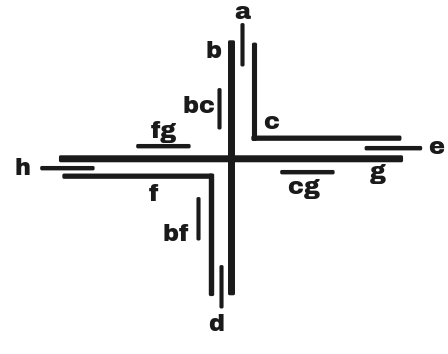
\includegraphics[width=4cm]{./img/falsePie.png}  %\label{fig:falsePie} 
    & &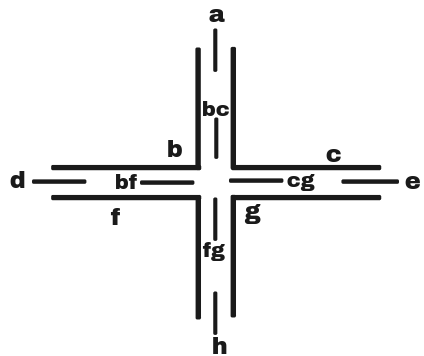
\includegraphics[width=4cm]{./img/truePie.png} %\label{fig:truePie}
    & &
 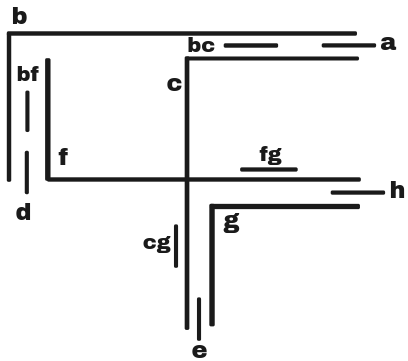
\includegraphics[width=4cm]{./img/frame.png} \\%[\abovecaptionskip]
    {\footnotesize (a) Baseada em torta falsa}  & &  {\footnotesize(b) Baseada em torta verdadeira} & & {\footnotesize (c) Baseada em moldura} %\label{fig:frame}
  \end{tabular}
  \caption{Diferentes representações de dobra simples para o grafo  $H$ utilizando uma  torta falsa (a), uma torta verdadeira (b) e uma moldura (c) para representar o $C_4^{H}$}\label{fig:falsepietruepieframe}
\end{figure} 

\begin{figure}[htb]	
\center%6.3
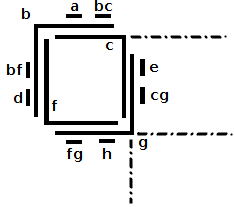
\includegraphics[width=4cm]{./img/outraRepresentacaoFrame3.png}
\caption{Uma representação por moldura onde as dobras dos caminhos pontilhados mudaram de sentido}
\label{fig:outraRepresentacaoFrame}
\end{figure}

\begin{definition}
Considere um grafo $G$ e um vértice $v \in V(G)$. Se em uma representação $B_1$-EPG de $G$ as duas arestas de dobra (ou uma aresta de extremidade) do caminho $P_v$ intersecta outros caminhos, então dizemos que  $P_v$ possui uma \emph{dobra obstruída (ou extremidade obstruída)}. 
Além do mais, dada uma representação $B_1$-EPG de $G$ onde $P_v$ possui uma dobra (ou extremidade) obstruída, dizemos que um subconjunto de caminhos \emph{obstrui} uma aresta de dobra (ou uma aresta de extremidade) de  $P_v$ se eles intersectam essa aresta. 
\end{definition}


\begin{fac} \label{fact:k24facts}
Em toda representação de dobra simples de um $K_{2,4}$, o caminho representando cada vértice do maior conjunto estável tem dobra em uma  torta falsa (ver mais em~\cite{Asinowski2009} e~\cite{daniel2014b}).
\end{fac}


\begin{lema}\label{lem:obstrucao}
Em qualquer representação de dobra simples do grafo  $G'$ retratado na  Figura~\ref{fig:extremidadeDobraObstruida}(a), o caminho $P_x$ possui extremidades e dobra obstruídos.
\end{lema}

\begin{proof}
Considere $G'$ consistindo de um vértice $x$, dois grafos isomorfos a  $H$, digamos $ H_1 $ e $ H_2 $, e um grafo bipartido $K_{2,4}$, tal que: $x$ é vértice do maior conjunto estável de $K_{2,4}$; $x$ é adjacente a um ciclo induzido de tamanho 3 de $H_1$, digamos $C_3^{H_1}$, e a um ciclo induzido de tamanho  3 de $H_2$, digamos $ C_3^{H_2}$, ver Figura~\ref{fig:extremidadeDobraObstruida}(a).

Sabemos que os caminhos pertencentes ao maior conjunto estável de um $K_{2,4}$ sempre dobram em uma  torta falsa, ver Fato~\ref{fact:k24facts}. Além disso $P_x$ é parte do maior conjunto estável desse  $K_{2,4}$, então $P_x$ possui uma \emph {dobra obstruída}, ver Figura~\ref{fig:extremidadeDobraObstruida}(b). 

O vértice  $x$ é adjacente ao $ C_{3}^{H_1}$ e ao $ C_3^{H_2}$, dessa forma o caminho $ P_x $ intersecta os caminhos representando eles. Mas em representações de dobra simples de um grafo isomorfo a $H$ existem pares de caminhos que sempre estão sobre o mesmo segmento de um raio central ou de uma intersecção de lado, ver o Corolário~\ref{coro:paresMesmoSegmento}, e a representação de  $C_{3}^{H_1}$ (similarmente para $C_3^{H_2})$ possui um desses caminhos. Todavia, existe uma aresta no conjunto de caminhos que representam  ${H_1}$ (similarmente em ${H_2}$) que tem uma intersecção de   3 caminhos representando $ C_{3}^{H_1}$ (e $ C_3^{H_2}$), caso contrário a representação não seria Helly, e existe  uma outra aresta distinta no mesmo  raio central ou intersecção de lado que é intersectada por três outros caminhos diferentes onde pelo menos um deles é diferentes dos caminhos correspondentes a $C_{3}^{H_1}$ (similarmente $C_3^{H_2}$). Assim, em uma representação de dobra simples de  $G'$, os caminhos que representam  $C_{3}^{H_1}$ (similarmente $C_3^{H_2})$ devem intersectar uma aresta de dobra ou uma aresta de extremidade de $P_x$, porque $P_x$ intersecta somente um dos conjuntos de caminhos que estão sobre o mesmo raio central ou intersecção de lado onde  $C_{3}^{H_1}$ (similarmente $C_3^{H_2})$ está. Como a dobra de   $P_x$ já está obstruída pelo restante da estrutura de $K_{2,4}$, então ${H_1}$ (similarmente ${H_2}$) deve estar posicionado na aresta de extremidade de  $P_x$. Isso implica que  $ P_x $ possui uma condição de \emph{extremidades obstruídas} e \emph{dobra obstruída}, ver Figura~\ref{fig:extremidadeDobraObstruida}(b).
\begin{figure}[h]
  \centering
  \begin{tabular}{p{6cm} p{1cm} p{6cm}}
     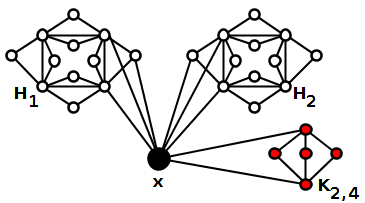
\includegraphics[width=5cm, center]{./img/grafoDobraExtremidadeObstruida2.png} &  &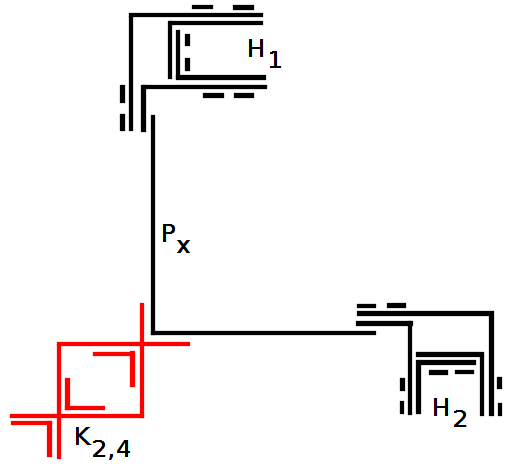
\includegraphics[width=6cm, center]{./img/extremidadeDobraObstruida5.png}  \\%[\abovecaptionskip]
    \footnotesize \centering (a) O grafo $G'$& & \footnotesize \centering (b)Uma representação $B_1$-EPG de $G'$%\\
 %   &&
  \end{tabular}
 \caption{Um exemplo de extremidade e dobra obstruída.} \label{fig:extremidadeDobraObstruida}
\end{figure}
\end{proof}




\begin{definition}
Dizemos que um segmento $s$ está \emph{internamente contido} em um caminho $P_x$ se $s$ está contido em $P_x$, e ele não intersecta uma aresta relevante de  $P_x$. 
\end{definition}

% \begin{fac}
% In a single bend representation of a graph, if a path $p(y)$ has an obstructed bend and obstructed extremities, and some path $p(x)$ intersects $p(y)$, but does not intersect paths that obstruct the extremities and the bend edges of $p(y)$, then the intersection between $p(x)$ and $p(y)$ isinternamente contida into $p(y)$. 
% \end{fac}


\begin{lema}\label{lem:volta}
Se um grafo $G_F$, construído de acordo com a definição  Definição~\ref{sec:reducao}, admite uma representação $B_1$-EPG-Helly, então a CNF-fórmula $F$ associada é uma instância-sim de {\sc Positive (1 in 3)-3sat}.
\end{lema}

% \setcounter{prove}{3}
\begin{proof}
Suponha que $G_F$ possui uma representação $B_1$-EPG-Helly, $R_{G_F}$. A partir de $R_{G_F}$ construiremos uma atribuição que satisfaz $F$. 

Primeiro, note que em toda representação de dobra simples de um $K_{2,4}$, o caminho de cada vértice do maior conjunto estável, em particular $P_{T}$ (em $R_{G_F}$), possui dobras contidas em uma torta falsa (ver Fato~\ref{fact:k24facts}). 


O vértice  $T$ é adjacente aos vértices de um triângulo de  $G_{B1}$ e $G_{B2}$. Como o $K_{2,4}$ está posicionado na dobra de  $P_{T}$, então em $R_{G_F}$ a representação de $G_{B1}$ e $G_{B2}$ devem ser posicionadas nas extremidades de $P_{T}$, ver Lema~\ref{lem:obstrucao}.   


Sem perda de generalidade, considere que $P_{V} \cap P_{T}$ é um segmento horizontal em $R_{G_F}$.

Podemos notar em $R_{G_F}$ que: o número de caminhos $P_{d}$ com segmento internamente contido em  $P_{V}$ é exatamente o número de cláusulas em $F$; a intersecção entre cada  $P_{a}, P_{e}, P_{h}$ no  dispositivo cláusula e cada caminho $P_{v_j}$ indica as variáveis que compõem a cláusula. Assim, podemos atribuir para cada variável $ x_{j}$ o valor \textit{True} se a aresta intersectante entre $P_{v_j}$ e $P_{T}$ é horizontal, e \textit{False} caso contrário. 


No Lema~\ref{lem:2vertical2horizontal} foi mostrado que qualquer representação minimal $B_1$-EPG de um dispositivo cláusula possui dois caminhos em $\{P_{a}, P_{d}, P_{e}, P_{h}\}$ com direção vertical e outros dois caminhos possuem direção horizonal. Além disso $P_{d}$ intersecta $P_{V}$, segue-se que em uma representação de dobra simples de  $G_F$ devemos conectar dois desses caminhos de forma a representar uma atribuição $False$, e exatamente um representará uma atribuição $True$. Assim, mostramos que a partir de $R_{G_F}$ podemos obter uma atribuição para $F$ tal que toda cláusula possui exatamente uma variável com valor $True$.
 \end{proof}


Note que uma representação $B_1$-EPG é  Helly se e somente se cada clique é representada por uma  clique-aresta (e não por uma  clique-garra). Mais detalhes sobre clique-aresta e clique-garra podem ser encontrados em~\cite{golumbic2009}. Assim, uma maneira alternativa para checar que uma representação é Helly seria notar que todas as cliques estão representadas como cliques-aresta.

\smallskip

Alguns vértices de  $G_F$ tem representação $B_1$-EPG altamente restritiva. O vértice $T$ possui sua dobra e ambas extremidades obstruídas por seus vizinhos, subgrafos $G_{B1}$, $G_{B2}$ e o restante do grafo $K_{2,4}$. O vértice $V$ e cada  vértice-variável $v_i$ deve ter um de seus segmentos internamente contigo em  $T$, e também suas extremidades e dobra obstruídos.  Portanto, o vértice $V$ e cada 
vértice-variável possui somente um segmento cada que pode ser utilizado em uma representação EPG para fazer a adjacência deles ao dispositivo cláusula. A direção desse segmento, começando pela horizontal ou vertical, pode ser utilizado para representar uma valoração $True$ ou $False$ para as variáveis. O  dispositivo cláusula, por outro lado, é tal que exatamente duas de suas adjacências aos vértices-variável e a $V$ pode ser efetuada com uma intersecção horizontal enquanto as outras duas  devem ser realizadas com intersecção vertical. Se considerarmos a direção utilizada por  $V$ como uma atribuição verdadeira, podemos notar que exatamente uma das variáveis em cada cláusula será $True$ em qualquer possível representação de  $G_F$. Por outro lado, é razoavelmente simples obter uma representação $B_1$-EPG para $G_F$ dada uma atribuição verdadeira para a fórmula $F$.


\begin{theorem}
{\sc Reconhecimento de grafos $B_{1}$-EPG-Helly } é NP-completo.
\end{theorem}
\begin{proof}
Pelo Teorema~\ref{teo:nppertinencia} e Lemas~\ref{lem:ida} e~\ref{lem:volta}.
 \end{proof} %$\square$

Dizemos que um grafo $k$-apex é um grafo que pode ser feito planar pela remoção de $k$ vértices. Além do mais, um grafo $d$-degenerado é um grafo em que todo subgrafo possui um vértice de grau no máximo $d$. Lembrando que  {\sc Positive (1 in 3)-3SAT} permanece $NP$-completo quando o grafo de incidência da fórmula de entrada é planar~\cite{mulzer2008minimum}. Assim, o seguinte corolário é válido.

\begin{corollary}
 \label{coro:2apexAnd3degenerate}
{\sc Reconhecimento de grafos $B_{1}$-EPG-Helly} é NP-completo sobre grafos $2$-apex e $3$-degenerado.
\end{corollary}

\begin{proof}
É fácil ver que os grafos construídos de acordo com a Definição~\ref{sec:reducao} são $3$-degenerados.
Como {\sc Positive (1in3)-3SAT} permanece $NP$-completo quando o grafo de incidência da fórmula  $F$ é planar~\cite{mulzer2008minimum},  de uma instância $F$ de {\sc Planar Positive (1in3)-3SAT}, então usando uma representação planar do grafo de incidência de $F$, podemos observar que pela remoção de $V$ e $T$ de $G_F$ obtemos um grafo planar. Logo, $G_F$ é 2-apex. 
\end{proof}


Para provar que $G_F$ é 3-degenerado basta aplicar o algoritmo de reconhecimento de grafos $d$-degenerados, que consiste em repetidamente remover os vértices de grau mínimo do grafo. Note que o vértice a ser removido a cada iteração do algoritmo sempre possui grau no máximo três, e portanto $G_F$ é 3-degenerado.

%Para elucidar o Corolário~\ref{coro:2apexAnd3degenerate}, que pode não ser trivial, sugerimos o seguinte raciocínio para provar que $G_F$ é 3-degenerado: aplicar o algoritmo de reconhecimento de grafos $d$-degenerados. 
A título de exemplo apresentamos a seguir uma construção para esclarecer a segunda parte do corolário. Tomemos a fórmula $F=(x_1+x_2+x_3)\wedge(x_1+x_3+x_4)\wedge(x_1+x_2+x_4)$, que  é uma instância de {\sc Planar Positive (1in3)-3SAT} e vamos mostrar que o dispositivo específico $G_F$ gerado a partir dessa instância é um grafo 2-apex.

Primeiro, monte o grafo de incidência de $F$, chamemos ele de $I_F$. O grafo de incidência é um grafo bipartido onde uma das partições está relacionada com as cláusulas de $F$ e a outra partição está relacionada com as suas variáveis. Cada cláusula $C_i$ de $F$ é representada por um vértice $v_{c_i}$ e cada variável $x_j$ das cláusulas é representada por um vértice $v_{x_j}$. Uma aresta  $(v_{c_i}, v_{x_j})$ existe em $I_F$ se e somente se a variável $x_j$ ocorre na cláusula $C_i$. A Figura~\ref{fig:grafoIncidencia2apex} retrata uma construção do grafo de incidência $I_F$.

\begin{figure}[htb]	
\center%6.3
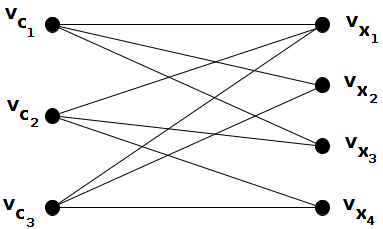
\includegraphics[width=6cm]{./img/grafoIncidencia2apex.png}
\caption{Grafo de incidência $I_F$, formato bipartição }
\label{fig:grafoIncidencia2apex}
\end{figure}

Como a fórmula $F$ que originou o grafo $I_F$ é uma instância de {\sc Planar Positive (1in3)-3SAT}, sabemos que o grafo de incidência da fórmula  $F$ é também planar~\cite{mulzer2008minimum}. A Figura~\ref{fig:grafoIncidencia2apexPlanar} retrata uma representação planar de $I_F$.


\begin{figure}[htb]	
\center%6.3
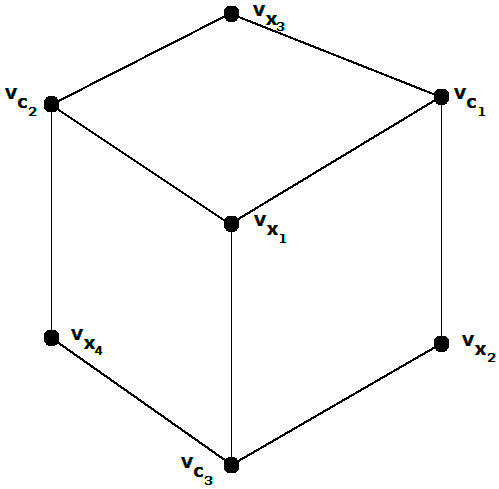
\includegraphics[width=8cm]{./img/grafoIncidencia2apexPlanar.png}
\caption{Grafo de incidência $I_F$ em uma representação planar }
\label{fig:grafoIncidencia2apexPlanar}
\end{figure}

Finalmente, podemos substituir os vértices que representavam as variáveis e cláusulas em $I_F$ pelos dispositivos variáveis e cláusulas correspondentes. Os vértices $V$ e $T$ são removidos. Como cada dispositivo variável, dispositivo cláusula e dispositivo base individualmente era planar, então algo não planar pode ter surgido somente da intersecção que foi feita entre eles. Como $I_F$ garante que existe um arranjo planar entre as intersecções dos dispositivos variável e dispositivos cláusula, então quando removemos $V$ e $T$, tudo o que sobra do grafo é planar, ver Figura~\ref{fig:grafoIncidenciaCompleto}. Logo $G_F$ é 2-apex.


\begin{figure}[htb]	
\center%6.3
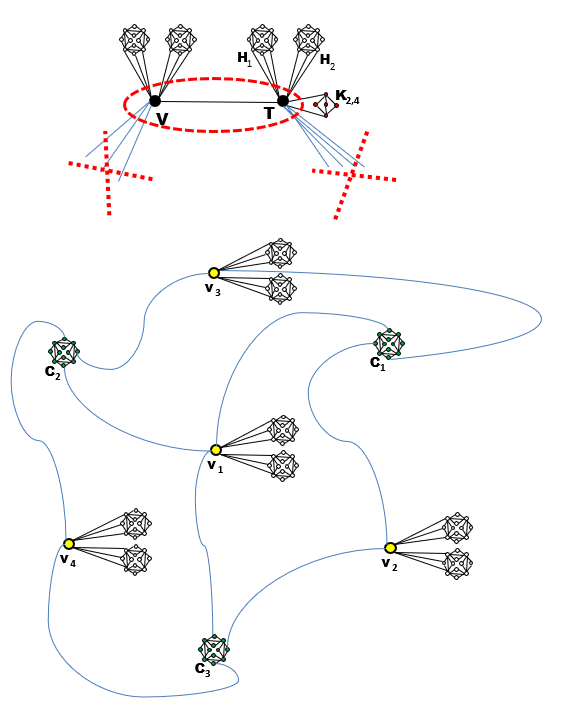
\includegraphics[width=10cm]{./img/grafoIncidenciaCompleto.png}
\caption{Grafo planar $G_F$, obtido a partir de $I_F$, a menos dos vértices $V$ e $T$ }
\label{fig:grafoIncidenciaCompleto}
\end{figure}





\section{Article accepted for publication in the journal  Discrete Mathematics \& Theoretical Computer Science} 
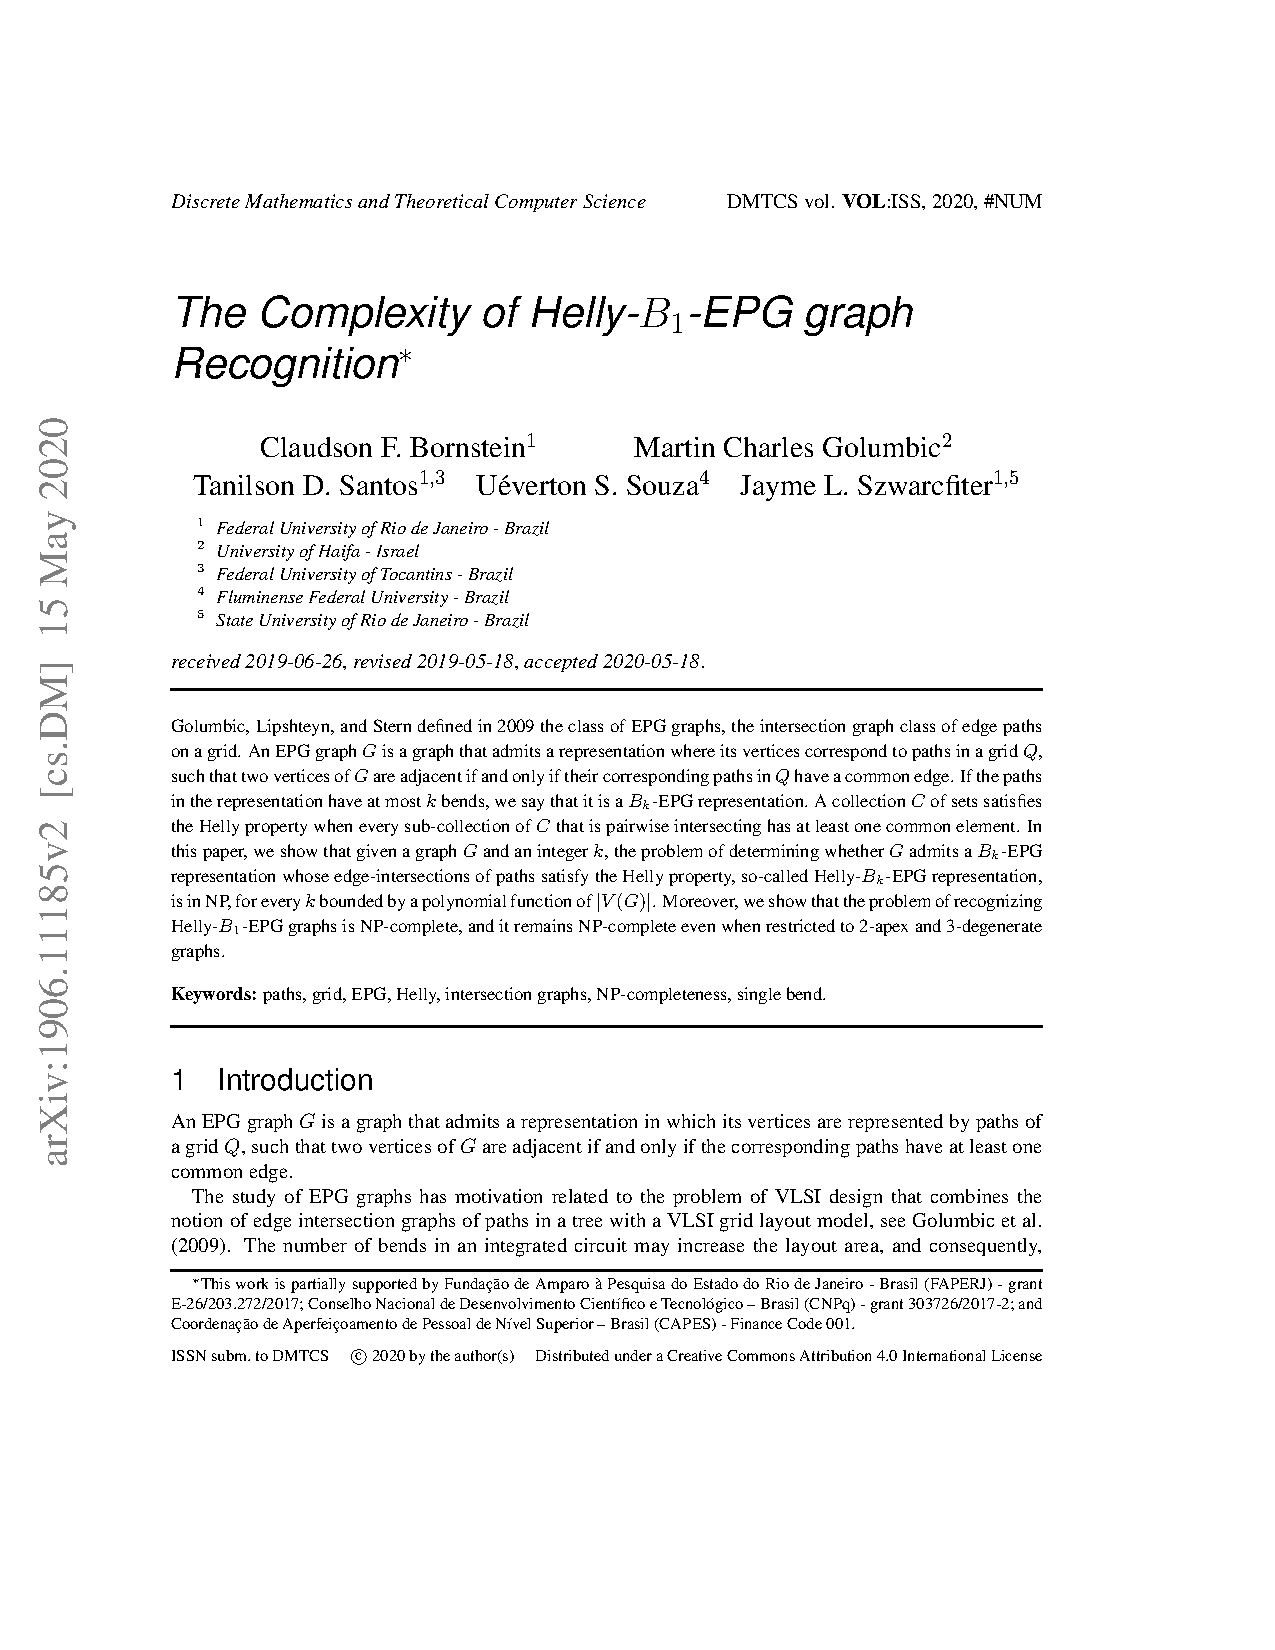
\includepdf[pages=-]{./includes/include-pdf-files/dmtcsTanilson.pdf}